\subsection{\texorpdfstring{连续映射空间中的 \(\mathfrak{S}\)-收敛}{连续映射空间中的 S-收敛}}

设 X、Y 为两个拓扑空间，用 C(X; Y) 表示由 X 到 Y 中的全体连续映射所成之集。若 S 是 X 的子集所成之集，且 Y 是一致空间，则用 \(\mathcal{C}_{\mathfrak{S}}(\mathbf{X};\mathbf{Y})\) 表示赋有 S-收敛一致结构的集合 C(X; Y)。特别地，\(\mathcal{C}_{s}(\mathbf{X};\mathbf{Y})\) 、\(\mathcal{C}_{c}(\mathbf{X};\mathbf{Y})\) 与 \(\mathcal{C}_{u}(\mathbf{X};\mathbf{Y})\) 分别表示赋有逐点收敛、紧收敛与一致收敛一致结构的集合 C(X; Y)。

命题 6. 设 X 是拓扑空间，Y 是一致空间，S 是 X 的子集所成之集。对每个 A ∈ S 以及 Y 的每个闭围域 V，W(A, V) 与 W(A̅, V) 在 C (X; Y) × C (X; Y) 上的迹相同。

因为若 \(u, v\) 是 \(\mathbf{X}\) 到 \(\mathbf{Y}\) 中的连续映射，则映射 \(x \to (u(x), v(x))\) 把 \(\mathbf{X}\) 映入 \(\mathbf{Y} \times \mathbf{Y}\) 并且连续，于是由 \((u(x), v(x)) \in \mathbf{V}\) 对一切 \(x \in \mathbf{A}\) 成立这一假设便可推出，\((u(x), v(x)) \in \overline{\mathbf{V}} = \mathbf{V}\) 对一切 \(x \in \overline{\mathbf{A}}\) 成立（第 I 章，§ 2，第 1 号，定理 1）。

若用 \(\overline{\mathfrak{S}}\) 表示在 \(\mathbf{X}\) 中所取的 \(\mathfrak{S}\) 的诸集的闭包所成之集，则命题 6 表明，在 \(\mathcal{C}(\mathbf{X};\mathbf{Y})\) 上，\(\mathfrak{S}\) -收敛与 \(\overline{\mathfrak{S}}\) -收敛的结构相同。

推论. 设 B 是 X 的稠密子集。在 C(X; Y) 上，一致收敛的结构与 B 上的一致收敛的结构相同。

命题 7. 设 X 是拓扑空间，S 是 X 的子集所成之集，Y 是一致空间。若 Y 是豪斯多夫空间，且 S 中诸集的并 B 在 X 中稠密，则 \(\mathcal{C}_{\mathfrak{S}}(X;Y)\) 是豪斯多夫空间。

因为若 \((u, v)\) 属于所有的集 \(W(A, V)\) ，其中 \(A \in \mathfrak{S}\) 而 \(V\) 取遍 \(Y\) 的围域，则由 \(Y\) 是豪斯多夫空间这一假设知，\(u(x) = v(x)\) 对一切 \(x \in B\) 成立；若 \(u\) 与 \(v\) 连续，则由恒等延拓原理得 \(u = v\)（第 I 章，§ 8，第 1 号，命题 2 的推论 1）。

特别地，在 \(\mathcal{C}(\mathbf{X};\mathbf{Y})\) 上，\(\mathbf{X}\) 的一个稠密子集上的逐点收敛拓扑是豪斯多夫的。

命题 8. 设 X 是一个集合，F 是 X 上的滤子，Y 是一致空间。则由映射 \(u: \mathbf{X} \to \mathbf{Y}\) （其中 \(u(\mathfrak{F})\) 是 Y 上的柯西滤子基）所成之集 H 在 \(\mathcal{F}_u(\mathbf{X}; \mathbf{Y})\) 中是闭的。

设 \(u_0: \mathbf{X} \to \mathbf{Y}\) 属于 \(\mathbf{H}\) 在 \(\mathcal{F}_u(\mathbf{X}; \mathbf{Y})\) 中的闭包。设 \(\mathbf{V}\) 为 \(\mathbf{Y}\) 的任一对称围域，则存在映射 \(u \in \mathbf{H}\) ，使得 \((u_0(x), u(x)) \in \mathbf{V}\) 对一切 \(x \in \mathbf{X}\) 成立；另一方面，由假设存在集 \(\mathbf{M} \in \mathfrak{F}\) ，使得 \((u(x), u(x')) \in \mathbf{V}\) 每当 \(x\) 与 \(x'\) 都属于 \(\mathbf{M}\) 。由于 \((u_0(x), u(x)) \in \mathbf{V}\) 且 \((u_0(x'), u(x')) \in \mathbf{V}\) ，便得 \((u_0(x), u_0(x')) \in \overset{3}{\mathbf{V}}\) 每当 \(x\) 与 \(x'\) 都属于 \(\mathbf{M}\) ，从而 \(u_0(\mathfrak{F})\) 是 \(\mathbf{Y}\) 上的柯西滤子基。

推论 1. 设 X 是拓扑空间，Y 是一致空间。在一点 \(x_{0} \in X\) 处连续的、由 X 到 Y 中的映射所成之集在 \(\mathcal{F}_{u}(X; U)\) 中是闭的。

若 V 是 \(x_{0}\) 在 X 中的邻域滤子，则 \(u(x_{0})\) 是 \(u(\mathbf{V})\) 的接触点；因此 u 在 \(x_{0}\) 处连续当且仅当 \(u(\mathbf{V})\) 是 Y 上的柯西滤子基（第 II 章，§ 3，第 2 号，命题 5 的推论 2）。

推论 2. 设 X、L 为两个集合，分别带有滤子 F、G，并设 Y 是完备一致空间。对每个 \(\lambda \in L\) ，设 \(u_{\lambda}\) 是 X 到 Y 中的一个映射。假设：(i) 族 \((u_{\lambda})_{\lambda \in L}\) 在 X 中（关于滤子 G）一致收敛于映射 \(v: X \to Y\) ；(ii) 对每个 \(\lambda \in L\) ，\(u_{\lambda}\) 关于滤子 F 有极限 \(y_{\lambda}\) 。在这些条件下，\(v\) 关于 F 有极限，且 \(v\) 关于 F 的每个极限都是族 \((y_{\lambda})_{\lambda \in L}\) 关于 G 的极限。

因为 \(v\) 属于诸 \(u_{\lambda}\) 所成之集在 \(\mathcal{F}_u(\mathbf{X};\mathbf{Y})\) 中的闭包，故由命题 8 知 \(v(\mathfrak{F})\) 是 \(\mathbf{Y}\) 上的柯西滤子基；这表明 \(v\) 有极限 \(y\) （关于 \(\mathfrak{F}\) ），因为 \(\mathbf{Y}\) 是完备的。设

\(X' = X \cup \{\omega\}\) 为与滤子 \(\mathfrak{F}\) 相伴的拓扑空间（第 I 章，§ 6，第 5 号），并把 \(u_{\lambda}\) （相应地，\(v\) ）延拓为 \(\overline{u}_{\lambda}\) （相应地，\(\overline{v}\) ），即 \(X'\) 到 Y 中的映射，办法是令 \(\overline{u}_{\lambda}(\omega) = y_{\lambda}\) {[}相应地 \(\overline{v}(\omega) = y\) {]}。于是映射 \(\overline{u}_{\lambda}, \overline{v}\) 在 \(X'\) 上连续，且 \(\overline{u}_{\lambda}\) 在 X 中一致收敛于 \(\overline{v}\) （关于 \(\mathfrak{G}\) ）；由于 X 在 \(X'\) 中稠密，命题 6 的推论表明 \(\overline{u}_{\lambda}\) 在 \(X'\) 中一致收敛于 \(\overline{v}\) ，特别地有 \(y = \lim_{\mathfrak{G}} y_{\lambda}\) 。

定理 2. 设 X 是拓扑空间，Y 是一致空间。则由 X 到 Y 中的连续映射所成之集 C(X; Y) 是赋有一致收敛拓扑的空间 F(X; Y) 的闭子集。

对每个 \(x \in \mathbf{X}\) ，由 \(\mathbf{X}\) 到 \(\mathbf{Y}\) 中的、在 \(x\) 处连续的映射所成之集在 \(\mathcal{F}_u(\mathbf{X};\mathbf{Y})\) 中是闭的（命题 8 的推论 1）；因此这些集的交 \(\mathcal{C}(\mathbf{X};\mathbf{Y})\) 也是闭的。

这一结果可以表述为：连续函数的一致极限仍然连续。

推论 1. 若 Y 是完备一致空间，则 \(\mathcal{C}_{u}(\mathbf{X};\mathbf{Y})\) 是完备的。因为由定理 2，\(\mathcal{C}_{u}(\mathbf{X};\mathbf{Y})\) 是一致空间 \(\mathcal{F}_{u}(\mathbf{X};\mathbf{Y})\) 的闭一致子空间，而后者由第 5 号的定理 1 是完备的。

推论 2. 设 X 是拓扑空间，S 是 X 的子集所成之集，Y 是一致空间。用 \(\tilde{\mathcal{C}}_{\mathfrak{S}}(X;Y)\) 表示由其在 S 的每个集上的限制都连续的、X 到 Y 中的全体映射所成之集。则 \(\tilde{\mathcal{C}}_{\mathfrak{S}}(X;Y)\) 是一致空间 \(\mathcal{F}_{\mathfrak{S}}(X;Y)\) 的闭子空间，且当 Y 完备时它是完备的。

设 \(u\) 属于 \(\tilde{\mathcal{C}}_{\mathfrak{S}}(\mathbf{X};\mathbf{Y})\) 在 \(\mathcal{F}_{\mathfrak{S}}(\mathbf{X};\mathbf{Y})\) 中的闭包；则（第 2 号）对每个 \(\mathbf{A} \in \mathfrak{S}\) ，\(u|\mathbf{A}\) 属于 \(\mathcal{C}(\mathbf{A};\mathbf{Y})\) 在 \(\mathcal{F}_u(\mathbf{A};\mathbf{Y})\) 中的闭包，从而由定理 2 知它连续。

推论 3. 设 X 是可度量化或局部紧的拓扑空间，Y 是一致空间。则 \(\mathcal{C}(\mathbf{X};\mathbf{Y})\) 在一致空间 \(\mathcal{F}_c(\mathbf{X};\mathbf{Y})\) 中是闭的；若此外 Y 还是完备的，则一致空间 \(\mathcal{C}_c(\mathbf{X};\mathbf{Y})\) 是完备的。

由推论 2，只需证明：若取 \(\mathfrak{S}\) 为 X 的紧子集所成之集，则在所考虑的两种情形下都有 \(\tilde{\mathcal{C}}_{\mathfrak{S}}(X;Y) = \mathcal{C}(X;Y)\) 。若 X 局部紧，这是显然的。若 X 可度量化，且 \(u: X \to Y\) 是一个在每个紧子集上的限制都连续的映射，则对每个 \(x \in X\) 以及每个序列 \((z_n)\) （由 X 的点组成且收敛于 \(x\) ），有 \(u(x) = \lim_{n \to \infty} u(z_n)\) ，因此 \(u\) 在 \(x\) 处连续（第 IX 章，§ 2，第 6 号，命题 10）。

注意，只要 \(\mathbf{X}\) 的每一点都具有可数的基本邻域系，上面的论证就适用。

\pandocbounded{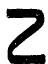
\includegraphics[keepaspectratio]{images/part002_71b18b59.jpg}}

注。1) 一般说来，集 \(\mathcal{C}(\mathbf{X};\mathbf{Y})\) 关于逐点收敛拓扑在 \(\mathcal{F}(\mathbf{X};\mathbf{Y})\) 中不是闭的：换句话说，连续函数的逐点极限未必连续{[}习题 5 a){]}。

\begin{enumerate}
\def\labelenumi{\arabic{enumi})}
\setcounter{enumi}{1}
\tightlist
\item
  \(\mathcal{C}(\mathbf{X};\mathbf{Y})\) 上的一个滤子可以逐点收敛于一个连续函数而不一致收敛于这个函数。
\end{enumerate}

例如，在区间 I = {[}0, 1{]} 上，设 \(u_n\) 是这样的实值函数：当 \(x = 0\) 且 \(2/n \leqslant x \leqslant 1\) 时等于 0，当 \(x = 1/n\) 时等于 1，并且在区间 {[}0, 1/n{]} 与 {[}1/n, 2/n{]} 的每一个中都是线性的。序列 \((u_n)\) 逐点收敛于 0，但在 I 中不一致收敛于 0（参见习题 6）。

\begin{enumerate}
\def\labelenumi{\arabic{enumi})}
\setcounter{enumi}{2}
\item
  若 X 是一致空间，则与命题 8 类似的证明表明，由 X 到 Y 中的一致连续映射所成之集在 \(\mathcal{F}_u(X;Y)\) 中是闭的。
\item
  设一致空间 Y 带有一个交换且结合的合成律，用加法记写，使得映射 \((y, y') \to y + y'\) 在 \(Y \times Y\) 上连续。于是，若 \((u_n)\) 是 X 到 Y 中的连续映射序列，且以 \(u_n\) 为通项的级数在 X 中一致收敛，则该级数的和在 X 上连续。
\end{enumerate}

关于连续映射的一致可和族（第 1 号，注 5）的相应结果，留给读者自行叙述。

命题 9. 设 X 是拓扑空间，Y 是一致空间。则映射 \((f, x) \to f(x)\) （由 \(\mathcal{C}_u(X; Y) \times X\) 到 Y 中）是连续的。

设 \(f_0: \mathbf{X} \to \mathbf{Y}\) 是连续映射，\(x_0\) 是 \(\mathbf{X}\) 的一点，\(\mathbf{V}\) 是 \(\mathbf{Y}\) 的一个围域。集 \(\mathbf{T}\) 由诸连续映射 \(f: \mathbf{X} \to \mathbf{Y}\) 组成，它们满足 \((f(x), f(x_0)) \in \mathbf{V}\) 对一切 \(x \in \mathbf{X}\) 成立；这个集是 \(f_0\) 在 \(\mathcal{C}_u(\mathbf{X}; \mathbf{Y})\) 中的一个邻域。另一方面，由于 \(f_0\) 连续，存在一个邻域 \(\mathbf{U}\) （\(x_0\) 在 \(\mathbf{X}\) 中的邻域），使得 \((f_0(x), f_0(x_0)) \in \mathbf{V}\) 对一切 \(x \in \mathbf{U}\) 成立。因此我们有 \((f(x), f(x_0)) \in \overset{\circ}{\mathbf{V}}\) 每当 \((f, x) \in \mathbf{T} \times \mathbf{U}\) ，从而结论得证。

\section{等度连续集}

\subsection{定义与一般判别法}

定义 1. 设 X 是拓扑空间，Y 是一致空间。称 F(X; Y) 的子集 H 在一点 \(x_{0} \in X\) 处等度连续，如果对 Y 的每个围域 V，存在 \(x_{0}\) 在 X 中的邻域 U，使得 \((f(x_{0}),f(x))\in\mathbf{V}\) 对一切 \(x\in\mathbf{U}\) 及一切 \(f\in\mathbf{H}\) 成立。称 H 是等度连续的，如果它在 X 的每一点都等度连续。

定义 2. 设 X 与 Y 是两个一致空间。称 \(\mathcal{F}(X;Y)\) 的子集 H 是一致等度连续的，如果对 Y 的每个围域 V，存在 X 的围域 U，使得我们就有 \((f(x), f(x')) \in V\) ，只要 \((x, x') \in U\) 且 \(f \in H\) 。

称 X 到 Y 中的映射的族 \((f_{t})_{t\in I}\) 在一点 \(x_0\) 处等度连续（相应地，等度连续、一致等度连续），如果诸 \(f_{t}\) 所成之集在 \(x_0\) 处等度连续（相应地，等度连续、一致等度连续）。

显然，若 \(\mathbf{H}\subset\mathcal{F}(\mathbf{X};\mathbf{Y})\) 在 \(x_{0}\) 处等度连续，则每个 \(f\in H\) 在 \(x_{0}\) 处连续；若 H 等度连续，则每个 \(f\in H\) 在 X 上连续，即 \(\mathbf{H}\subset\mathcal{C}(\mathbf{X};\mathbf{Y})\) 。同样，若 H 一致等度连续（X 是一致空间），则每个 \(f\in H\) 在 X 上一致连续。同样显然的是，一致等度连续的映射集是等度连续的；但一个由一致连续映射组成的集可以是等度连续的而非一致等度连续的（见习题 1；命题 1 的推论 2；以及第 2 号的命题 4）。

例。1) 设 X 是拓扑空间（相应地，一致空间），Y 是一致空间。由 X 到 Y 中的连续（相应地，一致连续）映射所成的每个有限集都是等度连续（相应地，一致等度连续）的。

\begin{enumerate}
\def\labelenumi{\arabic{enumi})}
\setcounter{enumi}{1}
\tightlist
\item
  设 X、Y 是两个度量空间，d（相应地，d'）是 X（相应地，Y）上的度量，并设 k、\(\alpha\) 是两个实数 \textgreater{} 0。则使
\end{enumerate}

\[
d ^ {\prime} (f (x), f (x ^ {\prime})) \leqslant k (d (x, x ^ {\prime})) ^ {\alpha}
\]

对每一对点 \(x, x'\) （属于 \(\mathbf{X}\) ）都成立的全体映射 f: X → Y 所成之集是一致等度连续的。例如，\(\mathbf{X}\) 到 \(\mathbf{Y}\) 的一个子集上的全体等距映射（第 IX 章，§ 2，第 2 号）是一致等度连续的。

* 设 H 是定义在区间 I ⊂ R 上的实值函数所成之集，这些函数在 I 上可微，且满足 \(|f'(x)| \leqslant k\) 对所有 \(x \in I\) 及所有 \(f \in H\) 成立。则 H 是一致等度连续的，因为若 \(x_{1}, x_{2}\) 是 I 的任意两点，则由中值定理，有 \(|f(x_{1}) - f(x_{2})| \leqslant k |x_{1} - x_{2}|\) 对每个 \(f \in H\) 成立。 *

\begin{enumerate}
\def\labelenumi{\arabic{enumi})}
\setcounter{enumi}{2}
\tightlist
\item
  设 G 是拓扑群，Y 是一致空间，\(f: \mathbf{G} \to \mathbf{Y}\) 是一致连续映射{[}G 赋有它的左一致结构（第 III 章，§ 3，第 1 号）{]}。对每个 \(s \in \mathbf{G}\) ，用 \(f_s\) 表示 G 到 Y 中的映射 \(x \to f(sx)\) 。则诸映射 \(f_s(s \in \mathbf{G})\) 所成之集是一致等度连续的，因为关系 \(x^{-1}x' \in V\) 等价于 \((sx)^{-1}(sx') \in V\) 。
\end{enumerate}

命题 1. 设 T 是一个集合，S 是 T 的子集所成之集，Y 是一致空间，X 是拓扑（相应地，一致）空间，f 是 \(\mathbf{T} \times \mathbf{X}\) 到 \(\mathbf{Y}\) 中的一个映射。对每个 \(\mathbf{A} \in \mathfrak{S}\) ，用 \(\mathbf{H}_{\mathbf{A}} \subset \mathcal{F}(\mathbf{X}; \mathbf{Y})\) 表示诸映射 \(x \to f(t, x)\) （ \(t\) 取遍 \(\mathbf{A}\) ）所成之集。则映射 \(x \to f(., x)\) （由 \(\mathbf{X}\) 到 \(\mathcal{F}_{\mathfrak{S}}(\mathbf{T}; \mathbf{Y})\) 中）在一点 \(x_0 \in \mathbf{X}\) 处连续（相应地，一致连续）当且仅当集 \(\mathbf{H}_{\mathbf{A}}\) 在 \(x_0\) 处等度连续（相应地，一致等度连续）对一切 \(\mathbf{A} \in \mathfrak{S}\) 成立。

先考虑 \(\mathfrak{S} = \{\mathrm{T}\}\) ，即 \(\mathcal{F}_{\mathfrak{S}}(\mathrm{T};\mathrm{Y}) = \mathcal{F}_u(\mathrm{T};\mathrm{Y})\) 这一特殊情形。对 Y 的每个围域 V，条件 \((f(.,x),f(.,x'))\in W(\mathrm{V})\) 的意思是 \((f(t,x),f(t,x'))\in \mathrm{V}\) 对一切 \(t\in \mathrm{T}\) 成立。因此，说 \(x\to f(.,x)\) 在 \(x_0\) 处连续（相应地，一致连续）等价于说：对 Y 的每个围域 V，存在 \(x_0\) 在 X 中的邻域 U（相应地，X 的围域 M），使得关系 \(x\in \mathrm{U}\) {[}相应地 \((x,x')\in \mathrm{M}]\) 蕴涵 \((f(t,x),f(t,x_0))\in \mathrm{V}\) {[}相应地 \((f(t,x),f(t,x'))\in \mathrm{V}]\) 对一切 \(t\in \mathrm{T}\) 成立，于是命题由定义 1 与定义 2 得出。在一般情形，依 § 1，第 2 号，我们要表述的是：对每个 \(\mathrm{A}\in \mathfrak{S}\) ，映射 \(x\rightarrow f(.,x)|\mathrm{A}\) （由 X 到 \(\mathcal{F}_u(\mathrm{A};\mathrm{Y})\) 中）在 \(x_0\) 处连续（相应地，一致连续）；由前所述，这等价于说，对每个 \(\mathrm{A}\in \mathfrak{S}\) ，\(\mathrm{H}_{\mathrm{A}}\) 在 \(x_0\) 处等度连续（相应地，一致等度连续）。

把命题 1 应用于 \(\mathbf{T} = \mathbf{H}\) 且 \(f\) 是映射 \((h, x) \to h(x)\) （由 \(\mathbf{H} \times \mathbf{X}\) 到 \(\mathbf{Y}\) 中）的情形，便可把定义 1 与定义 2 改写成有时有用的形式；由于 \(f(., x)\) 是映射 \(h \to h(x)\) （由 \(\mathbf{H}\) 到 \(\mathbf{Y}\) 中），我们得到：

推论 1. 设 X 是拓扑（相应地，一致）空间，Y 是一致空间，H 是 \(\mathcal{F}\) (X; Y) 的子集。对每个 \(x \in \mathbf{X}\) ，用 \(\tilde{x}\) 表示 H 到 Y 中的映射 \(h \to h(x)\) 。则 H 在 \(x_0\) 处等度连续（相应地，一致等度连续）当且仅当映射 \(x \to \tilde{x}\) （由 X 到一致空间 \(\mathcal{F}_u\) (H; Y) 中）在 \(x_0\) 处连续（相应地，一致连续）。

特别地，若 X 是紧的，则 X 到 \(\mathcal{F}_{u}(H;Y)\) 中的每个连续映射都一致连续（第 II 章，§ 4，第 1 号，定理 2）。因此：

推论 2. 设 X 是紧空间，Y 是一致空间。则 \(\mathcal{F}(X;Y)\) 的每个等度连续子集都是一致等度连续的。

现在设有一个集合 T、一个拓扑空间 X、一个一致空间 Y 以及一个映射 \(f: T \times X \to Y\) 。用 \(\tilde{f}\) 表示映射 \(x \to f(., x)\) （由 X 到 \(\mathcal{F}_{u}(T; Y)\) 中），并考虑典型映射 \(\theta: (t, g) \to g(t)\) （由 \(T \times \mathcal{F}_{u}(T; Y)\) 到 Y 中）。显然，图表

\[
\mathrm{T} \times \mathrm{X} \xrightarrow {f} \mathrm{Y}
\]

\[
\iota_ {\mathrm{T}} \times \tilde {f} \searrow \nearrow \theta
\]

\[
\mathbf {T} \times \mathcal {F} _ {u} (\mathbf {T}; \mathbf {Y})
\]

（其中 \(\iota_{\mathbf{T}}\) 是 T 的恒等映射）是交换的。现在设 T 赋有一个拓扑，并且对每个 \(x \in \mathbf{X}\) ，映射 \(f(., x): t \to f(t, x)\) 连续；这时在上图中就可把 \(\mathcal{F}_{u}(\mathrm{T}; \mathrm{Y})\) 换成 \(\mathcal{C}_{u}(\mathrm{T}; \mathrm{Y})\) 。但由 § 1，第 6 号，命题 9 知 \(\theta\) 连续；因此若 \(\tilde{f}\) 连续，则 \(f\) 连续。由于 \(\tilde{f}\) 的连续性可以借助命题 1 来表达，我们得到下列结果：

推论 3. 设 T、X 是拓扑空间，Y 是一致空间，f 是 T × X 到 Y 中的一个映射。则 f 连续，只要下列条件满足：

\begin{enumerate}
\def\labelenumi{\arabic{enumi})}
\item
  对每个 \(x \in \mathbf{X}\) ，偏映射 \(t \to f(t, x)\) 连续。
\item
  当 \(t\) 取遍 \(\mathbf{T}\) 时，诸偏映射 \(x \to f(t, x)\) 组成 \(\mathfrak{F}(\mathbf{X}; \mathbf{Y})\) 的一个等度连续子集。
\end{enumerate}

特别地，取 T 为 \(\mathcal{F}(\mathbf{X};\mathbf{Y})\) 的一个子集 H，取 \(f\) 为典型映射 \((h,x)\to h(x)\) （由 \(\mathbf{H}\times \mathbf{X}\) 到 Y 中）；推论 3 的条件 1）意味着 H 赋有一个比逐点收敛拓扑更细的拓扑，而条件 2）意味着 H 等度连续。因此：

推论 4. 设 X 是拓扑空间，Y 是一致空间，H 是 X 到 Y 中的等度连续映射集。若 H 赋有逐点收敛拓扑，则映射 \((h, x) \to h(x)\) （由 \(H \times X\) 到 Y 中）连续。

更直观地，这表达了下列事实：若 \(h \in \mathbf{H}\) 逐点收敛于 \(h_0 \in \mathbf{H}\) ，且 \(x \in \mathbf{X}\) 收敛于 \(x_0\) ，则 \(h(x)\) 收敛于 \(h_0(x_0)\) 。

推论 5. 设 X 是拓扑空间，Y、Z 是两个一致空间，H 是 Y 到 Z 中的等度连续映射集。若 H、C(X; Y) 与 C(X; Z) 都赋有逐点收敛拓扑，则映射 \((u, v) \to u \circ v\) （由 H × C(X; Y) 到 C(X; Z) 中）连续。

我们必须证明，对每个 \(x \in \mathbf{X}\) ，映射 \((u, v) \to u(v(x))\) （由 \(\mathbf{H} \times \mathcal{C}(\mathbf{X}; \mathbf{Y})\) 到 \(\mathbf{Z}\) 中）连续。而 \(v \to v(x)\) 在 \(\mathbf{H}\) 上连续（ \(\S 1\) ，第 2 号，注 6），且由推论 4 知 \((u, y) \to u(y)\) 是 \(\mathbf{H} \times \mathbf{Y}\) 到 \(\mathbf{Z}\) 中的连续映射；由于 \((u, v) \to u(v(x))\) 是 \((u, y) \to u(y)\) 与 \((u, v) \to (u, v(x))\) 的复合，结论得证。

下面的命题及其推论是命题 1 的推论 3 与推论 4 关于一致等度连续映射集的类似结果：

命题 2. 设 T、X、Y 是一致空间，f 是 T × X 到 Y 中的一个映射。则 f 一致连续当且仅当下列两个条件满足：

\begin{enumerate}
\def\labelenumi{\arabic{enumi})}
\item
  诸映射 \(x \to f(t, x)\) （ \(t \in \mathbf{T}\) ）组成 \(\mathcal{F}(\mathbf{X}; \mathbf{Y})\) 的一个一致等度连续子集。
\item
  诸映射 \(t \to f(t, x)\) （ \(x \in \mathbf{X}\) ）组成 \(\mathcal{F}(\mathbf{T}; \mathbf{Y})\) 的一个一致等度连续子集。
\end{enumerate}

条件的必要性是容易看出的。反之，设它们成立。设 W 是 Y 的一个围域；则存在 T 的围域 U 与 X 的围域 V，使得：1） \((t', t'') \in \mathbf{U}\) 蕴涵：对每个 \(x \in X\) ，

\[
\left(f \left(t ^ {\prime}, x\right), f \left(t ^ {\prime \prime}, x\right)\right) \in W.
\]

\begin{enumerate}
\def\labelenumi{\arabic{enumi})}
\setcounter{enumi}{1}
\tightlist
\item
  \((x', x'') \in \mathbf{V}\) 蕴涵：对每个 \(t \in \mathbf{T}\) ，
\end{enumerate}

\[
(f (t, x ^ {\prime}), f (t, x ^ {\prime \prime})) \in W.
\]

现在显然，关系“ \((t', t'') \in \mathbf{U}\) 且 \((x', x'') \in \mathbf{V}\) ”蕴涵 \((f(t', x'), f(t'', x'')) \in \overset{2}{\mathbf{W}}\) ，由此即得结论。

特别地，取 T 为 \(\mathcal{F}(\mathbf{X};\mathbf{Y})\) 的一个子集 H（赋有一致收敛的一致结构），取 \(f\) 为典型映射 \((h,x)\to h(x)\) ；这时命题 2 的条件 2）自动满足，因为对 Y 的每个围域 W，由偶 \((h',h'')\) （满足 \((h'(x),h''(x))\in W\) 对一切 \(x\in X\) ）所成之集按定义是 H 的一致结构的一个围域。因此只需表述条件 1）；换句话说：

推论. 设 X、Y 是两个一致空间，H 是 \(\mathcal{F}(X;Y)\) 的一个子集。则 H 一致等度连续当且仅当映射 \((h,x) \to h(x)\) （由 \(H \times X\) 到 Y 中）一致连续，这里 H 赋有一致收敛的一致结构。

\subsection{等度连续性的特殊判别法}

显然，等度连续（相应地，一致等度连续）集的每个子集都是等度连续（相应地，一致等度连续）的。同样，若 X 是拓扑（相应地，一致）空间而 Y 是一致空间，则 \(\mathcal{F}(X;Y)\) 的等度连续（相应地，一致等度连续）子集的每个有限并都是等度连续（相应地，一致等度连续）的。

设 \(X, X'\) 是两个拓扑（相应地，一致）空间，\(Y, Y'\) 是两个一致空间，\(f: X \to X'\) 是连续（相应地，一致连续）映射，\(g: Y \to Y'\) 是一致连续映射。

由定义立即可知，映射 \(u \rightarrow g \circ u \circ f\) （由 \(\mathcal{F}(X; Y)\) 到 \(\mathcal{F}(X'; Y')\) 中）把等度连续（相应地，一致等度连续）集变换成等度连续（相应地，一致等度连续）集。

命题 3. 设 X 是拓扑（相应地，一致）空间，\((\mathbf{Y}_{t})_{t \in I}\) 是一致空间的一个族，Y 是一个集合，且对每个 \(t \in I\) ，设 \(f_{t}\) 是 Y 到 \(\mathbf{Y}_{t}\) 中的一个映射。给 Y 赋以使所有 \(f_{t}\) 都一致连续的最粗的一致结构。\(\mathcal{F}(\mathbf{X}; \mathbf{Y})\) 的子集 H 等度连续（相应地，一致等度连续）的必要充分条件是：对每个 \(t \in I\) ，H 在映射 \(u \to f_{t} \circ u\) 下的像是 \(\mathcal{F}(\mathbf{X}; \mathbf{Y}_{t})\) 的一个等度连续（相应地，一致等度连续）子集。

这是定义 1、定义 2 以及 Y 的围域的定义的直接推论。

命题 4. 设 X、Y 是两个一致空间，H 是 X 到 Y 中的一致连续映射所成之集。设 \(\hat{X}, \hat{Y}\) 分别是 X、Y 的豪斯多夫完备化，并用 \(\tilde{H}\) 表示诸映射 \(\hat{u}: \hat{X} \to \hat{Y}\) （当 \(u\) 取遍 H 时）所成之集（第 II 章，§ 3，第 7 号，命题 15）。则 H 一致等度连续当且仅当 \(\tilde{H}\) 一致等度连续。

我们回顾，图表

\[
\begin{array}{c} \mathbf {X} \xrightarrow {u} \mathbf {Y} \\ i \downarrow \quad \quad \quad \quad \quad \quad \quad \quad \quad \quad \quad \quad \quad j \\ \hat {\mathbf {X}} \xrightarrow {\hat {u}} \hat {\mathbf {Y}} \end{array}\tag{1}
\]

是交换的，其中 \(i\) 与 \(j\) 是典型映射；此外，\(\mathbf{X}\) （相应地，\(\mathbf{Y}\) ）的一致结构是它在 \(i\) （相应地，\(j\) ）下 \(\hat{\mathbf{X}}\) （相应地，\(\hat{\mathbf{Y}}\) ）的一致结构的原像。于是 \(\mathbf{H}\) 一致等度连续当且仅当它在映射 \(u \to j \circ u\) 下的像一致等度连续（命题 3），从而我们已可限于 \(\mathbf{Y}\) 是豪斯多夫且完备的情形；此外，若 \(\tilde{\mathbf{H}}\) 一致等度连续，则 \(\mathbf{H}\) 也一致等度连续，因为它是 \(\tilde{\mathbf{H}}\) 在映射 \(\hat{u} \to \hat{u} \circ i\) 下的像；因此剩下要证的是 \(\mathbf{Y} = \hat{\mathbf{Y}}\) 时的逆命题。设 \(\mathbf{V}\) 是 \(\mathbf{Y}\) 的一个闭围域；由假设存在围域 \(\mathbf{U}\) （\(\mathbf{X}\) 的围域），使得关系 \((x, x') \in \mathbf{U}\) 与 \(u \in \mathbf{H}\) 蕴涵 \((u(x), u(x')) \in \mathbf{V}\) 。现在，若 \(\mathbf{U}'\) 是 \(\mathbf{U}\) 在 \(i \times i\) 下的像，则闭包 \(\overline{\mathbf{U}'}\) （\(\mathbf{U}'\) 在 \(\hat{\mathbf{X}} \times \hat{\mathbf{X}}\) 中的闭包）是 \(\hat{\mathbf{X}}\) 的一个围域（第 II 章，§ 3，第 7 号，命题 12）；假设表明，每当 \((z, z') \in \mathbf{U}'\) 且 \(u \in \mathbf{H}\) ，就有 \((\hat{u}(z), \hat{u}(z')) \in \mathbf{V}\) 。由于 \(\mathbf{V}\) 是闭的且 \(\hat{u}\) 连续，我们还有 \((\hat{u}(t), \hat{u}(t')) \in \mathbf{V}\) 对一切 \((t, t') \in \overline{\mathbf{U}'}\) 及一切 \(u \in \mathbf{H}\) 成立；证明完毕。

命题 5. 设 G、G' 是两个赋有各自左一致结构的拓扑群，H 是 G 到 G' 中的同态所成之集。则下列条件等价：

\begin{enumerate}
\def\labelenumi{\alph{enumi})}
\item
  H 在 G 的单位元 e 处等度连续，
\item
  H 等度连续，
\item
  H 一致等度连续。
\end{enumerate}

只需证明 a）蕴涵 c）。设 \(V'\) 是单位元 \(e'\) （\(G'\) 的单位元）的一个邻域；则由假设，存在 G 中 e 的邻域 V，使得 \(u(V) \subset V'\) 对一切 \(u \in H\) 成立；由于 H 的元素都是同态，关系 \(x^{-1}y \in V\) 蕴涵我们有

\[
(u (x)) ^ {- 1} u (y) = u (x ^ {- 1} y) \in \mathbf {V} ^ {\prime}.
\]

依据 G 与 G' 的左一致结构的围域的定义（第 III 章，§ 3，第 1 号），结论得证。

\subsection{等度连续集的闭包}

命题 6. 设 X 是拓扑（相应地，一致）空间，Y 是一致空间，H 是 \(\mathcal{F}(X;Y)\) 的一个子集。则 H 在一点 \(x_0 \in X\) 处等度连续（相应地，一致等度连续）当且仅当闭包 \(\overline{\mathbf{H}}\) （H 在 \(\mathcal{F}_s(X;Y)\) 中的闭包）在 \(x_0\) 处等度连续（相应地，一致等度连续）。

条件的充分性是显然的。为证必要性，考虑 Y 的一个在 \(Y \times Y\) 中为闭的围域 V；由假设，存在 X 中 \(x_{0}\) 的邻域 U（相应地，X 的围域 M），使得关系 \(x \in U\) （相应地，\((x', x'') \in M\) ）蕴涵 \((h(x_{0}), h(x)) \in V\) {[}相应地 \((h(x'), h(x'')) \in V\) {]}对一切 \(h \in H\) 成立。由于 V 是闭的，诸映射 \(h \in \mathcal{F}(X; Y)\) （满足关系 \((h(x_{0}), h(x)) \in V\) 对一切 \(x \in U\) {[}相应地，关系 \((h(x'), h(x'')) \in V\) 对一切 \((x', x'') \in M\) {]}）组成 \(\mathcal{F}_{s}(X; Y)\) 的一个闭子集（§ 1，第 2 号，注 6）；由于这个闭子集包含 H，它也包含 \(\overline{H}\) 。于是结论成立，因为 Y 的闭围域构成围域的一个基本系（第 II 章，§ 1，第 2 号，命题 2 的推论 2）。

\subsection{等度连续集上的逐点收敛与紧收敛}

定理 1. 设 X 是拓扑（相应地，一致）空间，Y 是一致空间，H 是 C(X;Y) 的一个等度连续（相应地，一致等度连续）子集。则 H 上的下列一致结构相同：紧（相应地，预紧）收敛的一致结构、逐点收敛的一致结构，以及在 X 的稠密子集 D 上逐点收敛的一致结构。

只需证明 H 上最后一个一致结构比第一个更细；换句话说，给定 Y 的一个围域 V 与 X 的一个紧（相应地，预紧）子集 A，存在 Y 的围域 W 与 D 的有限子集 F，使得关系

\[
u \in \mathrm{H}, \quad v \in \mathrm{H} \quad \text { and } \quad (u (x), v (x)) \in \mathrm{W} \quad \text { for   all } \quad x \in \mathrm{F}\tag{2}
\]

蕴涵

\[
(u (x), v (x)) \in \mathbf {V} \quad \text { for   all } \quad x \in \mathbf {A}.\tag{3}
\]

首先设 A 紧且 H 等度连续。给定 Y 的一个对称围域 W，每一点 \(x \in X\) 都有一个邻域 \(\mathrm{U}(x)\) ，使得关系 \(x' \in \mathrm{U}(x)\) 蕴涵 \((u(x), u(x')) \in \mathrm{W}\) 对一切 \(u \in H\) 成立。因此可以用有限个开集 \(U_i\) 覆盖紧集 A，使得对每一对点 \(x', x''\) （属于同一个集 \(U_i\) ），有 \((u(x'), u(x'')) \in \dot{\mathbf{W}}\) 对一切 \(u \in H\) 成立。设 \(a_i\) 是 \(D \cap U_i\) 的一个点，F 是诸 \(a_i\) 所成之集，并设（2）成立；则对每个 \(x \in A\) 存在一个指标 i，使得 \(a_i\) 与 x 属于同一集 \(U_i\) ，于是我们有 \((u(x), u(a_i)) \in \dot{\mathbf{W}}\) 与 \((v(a_i), v(x)) \in \dot{\mathbf{W}}\) ；这样，只要选取 W 使得 \(W \subset V\) ，（2）便蕴涵（3）。

若 A 预紧且 H 一致等度连续，我们就用第 2 号的命题 4；只需注意：\(i(\overline{\mathbf{A}})\) 在 \(\hat{\mathbf{X}}\) 中是紧的，\(i(\mathbf{D})\) 在 \(\hat{\mathbf{X}}\) 中稠密，以及 Y 的围域是 \(\hat{Y}\) 的围域在映射 \(j \times j\) 下的原像。

推论. 在定理 1 的假设下，闭包 \(\overline{\mathbf{H}}\) ——即 \(\mathbf{H}\) 在 \(\mathcal{F}(\mathbf{X};\mathbf{Y})\) 中关于逐点收敛拓扑的闭包——与 \(\mathbf{H}\) 在 \(\mathcal{C}(\mathbf{X};\mathbf{Y})\) 中关于紧（相应地，预紧）收敛拓扑的闭包相同。

因为由第 3 号的命题 6，集 \(\overline{H}\) 等度连续（相应地，一致等度连续），从而含于 C(X; Y)；结论立即由下列事实得出：依定理 1，在 \(\overline{H}\) 上所考虑的两个拓扑是相同的。

\subsection{连续映射的紧集}

定理 2（阿斯科利）. 设 X 是拓扑（相应地，一致）空间，S 是 X 的一个覆盖，Y 是一致空间，H 是 X 到 Y 中的映射所成之集，使得对每个 A ∈ S 及每个 u ∈ H，u 在 A 上的限制连续（相应地，一致连续）。则为使 H 关于 S-收敛的一致结构为预紧，下列条件在任何情形都是必要的，且当诸集 \(\mathbf{A} \in \mathfrak{S}\) 紧（相应地，预紧）时也是充分的：

\begin{enumerate}
\def\labelenumi{\alph{enumi})}
\item
  对每个 \(\mathbf{A} \in \mathfrak{S}\) ，集 \(\mathbf{H}|\mathbf{A} \subset \mathcal{F}(\mathbf{A};\mathbf{Y})\) （在 \(\mathbf{A}\) 上的、\(\mathbf{H}\) 中诸函数的限制）是等度连续（相应地，一致等度连续）的。
\item
  对每个 \(x \in \mathbf{X}\) ，集 \(\mathbf{H}(x) \subset \mathbf{Y}\) （由点 \(u(x)\) （ \(u \in \mathbf{H}\) ）组成）是预紧的。
\end{enumerate}

\begin{enumerate}
\def\labelenumi{\arabic{enumi})}
\tightlist
\item
  先证条件 a）与 b）是必要的。我们已知（§ 1，第 2 号，注 6）映射 \(u \to u(x)\) （由 \(\mathcal{F}_{\mathfrak{S}}(\mathbf{X};\mathbf{Y})\) 到 Y 中）是一致连续的；因此，若 H 预紧，则 \(\mathbf{H}(x)\) 也预紧（第 II 章，§ 4，第 2 号，命题 2），这就证明了 b）。为证 a），考虑一个集 \(\mathbf{A} \in \mathfrak{S}\) 、一点 \(x_0 \in \mathbf{A}\) 以及 Y 的一个围域 V；由于 H 预紧，它可以被有限个 \(W(\mathbf{A},\mathbf{V})\) -小的集所覆盖；换句话说，存在 H 中元素的一个有限序列 \((u_i)\) ，使得对每个 \(u \in \mathbf{H}\) ，我们有
\end{enumerate}

\[
(u (x), u _ {i} (x)) \in \mathbf {V} \quad \text { for   all } \quad x \in \mathbf {A}\tag{4}
\]

对至少一个指标 i 成立。

由于每个 \(u_{i}|A\) 都在 \(x_{0}\) 处连续（相应地，一致连续），存在邻域 \(U_{i}\) （\(x_{0}\) 在 A 中的邻域）（相应地，A 的一个围域 \(M_{i}\) ），使得

\[
x \in \mathrm{U} _ {i} \quad \text { implies } \quad (u _ {i} (x), u _ {i} (x _ {0})) \in \mathrm{V},\tag{5}
\]

（相应地，使得

\[
(x ^ {\prime}, x ^ {\prime \prime}) \in \mathbf {M} _ {i} \quad \text { implies } \quad (u _ {i} (x ^ {\prime}), u _ {i} (x ^ {\prime \prime})) \in \mathbf {V}.\tag{6}
\]

设 U（相应地，M）是诸 \(U_{i}\) （相应地，诸 \(M_{i}\) ）的交；它是 \(x_{0}\) 在 A 中的一个邻域（相应地，A 的一个围域）。对每个 \(u \in H\) 存在一个使（4）成立的指标 i；把条件（4）对 \(x_{0}\) 以及对 x（相应地，对 \(x'\) 与 \(x''\) ）写出，并注意到（5）{[}相应地（6）{]}，我们立即看出，关系 \(x \in U\) {[}相应地 \((x', x'') \in M\) {]}蕴涵 \((u(x), u(x_{0})) \in \overset{\mathbf{3}}{\mathrm{V}}\) {[}相应地 \((u(x'), u(x'')) \in \overset{\mathbf{3}}{\mathrm{V}}\) {]}对每个 \(u \in H\) 成立；这就证明了 a）。

\begin{enumerate}
\def\labelenumi{\arabic{enumi})}
\setcounter{enumi}{1}
\tightlist
\item
  现在证明：当诸集 \(A \in S\) 紧（相应地，预紧）时，条件 a）与 b）是充分的。条件 b）蕴涵 H 关于逐点收敛的一致结构是预紧的（第 II 章，§ 4，第 2 号，命题 3）。但由条件 a）与第 4 号的定理 1 可知，在 H\textbar A 上，A 中逐点收敛的一致结构与 A 中一致收敛的一致结构相同；因此 H\textbar A 在 \(\mathcal{F}_{u}(A; Y)\) 中是预紧的，这蕴涵 H 关于 S-收敛的一致结构是预紧的（§ 1，第 2 号）。
\end{enumerate}

注意，若 Y 是预紧空间，则定理 2 的条件 b）自动满足。

推论 1. 设 X 是拓扑（相应地，一致）空间，Y 是豪斯多夫一致空间，H 是 \(\mathcal{C}(\mathbf{X};\mathbf{Y})\) 的一个等度连续（相应地，一致等度连续）子集。假设 \(\mathrm{H}(x)\) 对每个 \(x\in \mathbf{X}\) 在 Y 中相对紧。则 H 在 \(\mathcal{C}(\mathbf{X};\mathbf{Y})\) 中关于紧（相应地，预紧）收敛拓扑是相对紧的。

设 \(\overline{\mathbf{H}}\) 是 \(\mathbf{H}\) 在 \(\mathcal{F}_s(\mathbf{X};\mathbf{Y})\) 中的闭包。\(\overline{\mathbf{H}}\) 是等度连续（相应地，一致等度连续）的（第 3 号，命题 6）。此外，我们有 \(\overline{\mathbf{H}}(x)\subset \overline{\mathbf{H}(x)}\) （ \(\S\) 1，第 2 号，注 6），因此 \(\overline{\mathbf{H}}(x)\) 也相对紧；于是定理 2 表明 \(\overline{\mathbf{H}}\) 关于 \(\mathfrak{S}\) -收敛是预紧的，这里 \(\mathfrak{S}\) 表示 \(\mathbf{X}\) 的所有紧（相应地，预紧）子集所成之集。此外，由于 \(\overline{\mathbf{H}(x)}\) 是紧的从而是完备的，\(\overline{\mathbf{H}}\) 关于逐点收敛的一致结构是完备的（第 II 章，\(\S\) 3，第 5 号，命题 10 以及第 4 号，命题 8），从而关于 \(\mathfrak{S}\) -收敛的一致结构也是完备的（ \(\S\) 1，第 5 号，命题 5 的推论 2）；于是 \(\overline{\mathbf{H}}\) 是紧的，因为它是预紧、完备且豪斯多夫的（ \(\S\) 1，第 2 号，命题 1）。

推论 2. 设 X 是拓扑（相应地，一致）空间，Y 是完备豪斯多夫一致空间，H 是 C(X; Y) 的一个等度连续（相应地，一致等度连续）子集。假设对一切 \(x \in D\) ，H(x) 在 Y 中相对紧，其中 D 是 X 的一个稠密子集。则 H 在 C(X; Y) 中关于紧（相应地，预紧）收敛拓扑是相对紧的。

只需证明 \(\mathrm{H}(x)\) 对一切 \(x \in X\) 相对紧，因为这样就可应用推论 1。由于 Y 完备，只需证明 \(\mathrm{H}(x)\) 对一切 \(x \in X\) 预紧。设 V 是 Y 的任一对称围域，则存在 x 的邻域 U，使得 \((u(x), u(x')) \in V\) 对一切 \(x' \in U\) 及一切 \(u \in H\) 成立。由假设存在 \(x' \in U \cap D\) ，且由于 \(\mathrm{H}(x')\) 在 Y 中相对紧，存在有限个点 \(y_k \in Y\) ，使得 \(\mathrm{H}(x')\) 含于诸集 \(\mathrm{V}(y_k)\) 的并；于是 \(\mathrm{H}(x)\) 含于诸集 \(\overset{2}{\mathrm{V}}(y_k)\) 的并，证明完毕。

推论 3. 设 X 是局部紧空间，Y 是豪斯多夫一致空间，H 是 C (X; Y) 的一个子集。则 H 在 \(\mathcal{C}_c(X; Y)\) 中相对紧当且仅当 H 等度连续且 H(x) 对一切 \(x \in \mathbf{X}\) 在 Y 中相对紧。

鉴于推论 1，只需证明：若 H 在 \(\mathcal{C}_{c}(\mathbf{X};\mathbf{Y})\) 中相对紧，则 H 等度连续。现在每一点 \(x\in X\) 都有一个紧邻域 A，且由定理 2 知 H/A 等度连续；这蕴涵 H 在 x 处等度连续，结论得证。

注。设 X 是拓扑空间，Y 是一致空间，S 是 X 的子集所成之集。则在 \(\mathcal{F}_{\mathfrak{S}}(X;Y)\) 的每个预紧子集 H 上，S-收敛的一致结构与在 \(B = \bigcup_{A \in \mathfrak{S}} A\) 中逐点收敛的一致结构相同。我们可以化到 \(B = X\) 且 Y 是豪斯多夫完备空间的情形；因为若 \(j\) 是典型单射 \(B \to X\) ，\(i\) 是典型映射 \(Y \to \hat{Y}\) ，则 \(\mathcal{F}(X;Y)\) 上的 S-收敛的一致结构是 \(\mathcal{F}(B;\hat{Y})\) 上的 S-收敛的一致结构在映射 \(\theta : u \to i \circ u \circ j\) 下的原像（ \(\S 1\) ，第 4 号，命题 4），且 H 预紧当且仅当 \(\theta(H)\) 预紧（第 II 章，\(\S 4\) ，第 2 号，命题 3）。在此情形，若 \(B = X\) 且 Y 是豪斯多夫完备空间，则 \(\mathcal{F}_{\mathfrak{S}}(X;Y)\) 是豪斯多夫且完备的（ \(\S 1\) ，第 2 号，命题 1 以及第 5 号，定理 1）；因此 H 在这个空间中的闭包 \(\overline{H}\) 是紧的。在 \(\overline{H}\) 上，逐点收敛拓扑是豪斯多夫的（ \(\S 1\) ，第 2 号，命题 1）且比 S-收敛拓扑粗；因此这两个拓扑相同（第 I 章，\(\S 9\) ，第 4 号，定理 2 的推论 3），从而 S-收敛与逐点收敛的一致结构也相同（第 II 章，\(\S 4\) ，第 1 号，定理 1）。

\section{特殊函数空间}

\subsection{映入度量空间的映射空间}

设 X 是一个集合，Y 是一致空间，\((f_{t})_{t\in I}\) 是定义 Y 的一致结构的伪度量族（第 IX 章，§ 1，第 4 号），S 是 X 的子集所成之集。对每个 \(t\in I\) 、每个集 \(A\in S\) 以及每对 X 到 Y 中的映射 \((u,v)\) ，记

\[
g _ {t, \mathrm{A}} (u, v) = \sup _ {x \in \mathrm{A}} f _ {t} (u (x), v (x));
\]

由此立即得出，\(g_{t,\mathbf{A}}\) 是 \(\mathcal{F}(\mathbf{X};\mathbf{Y})\) 上的一个伪度量，且伪度量族 \((g_{t,\mathbf{A}})_{t\in \mathbf{I},\mathbf{A}\in \mathfrak{S}}\) 定义了 \(\mathfrak{S}\) -收敛的一致结构（在 \(\mathcal{F}(\mathbf{X};\mathbf{Y})\) 上）。特别地：

命题 1. 若 Y 是可度量化的一致空间，则 \(\mathcal{F}(X;Y)\) 上的一致收敛的一致结构是可度量化的。

因为若 d 是 Y 上与其一致结构相容的一个度量，则 \(\mathcal{F}(X;Y)\) 上的一致收敛结构由单个伪度量

\[
\delta (u, v) = \sup _ {x \in \mathbf {X}} d (u (x), v (x));
\]

一般说来这个伪度量不是有限的，但它等价于一个有限伪度量（第 IX 章，§ 1，第 2 号）；由于一致收敛的一致结构是豪斯多夫的（§ 1，第 2 号，命题 1），故它是可度量化的。

推论. 设 X 是拓扑空间，Y 是可度量化的一致空间。假设存在 X 的紧子集的一个序列 \((\mathbf{K}_{n})\) ，使得 X 的每个紧子集都含于某个 \(K_{n}\) 。则 \(\mathcal{F}(\mathbf{X};\mathbf{Y})\) 上的紧收敛的一致结构是可度量化的。

由于诸 \(\mathbf{K}_n\) 覆盖 \(\mathbf{X}\) ，\(\mathcal{F}_c(\mathbf{X};\mathbf{Y})\) 同构于 \(\prod_{n}\mathcal{F}_{u}(\mathbf{K}_{n};\mathbf{Y})\) 的一个一致子空间（ \(\S 1\) ，第 2 号，注 3），因此该推论

由命题 1 得出（第 IX 章，§ 2，第 4 号，定理 1 的推论 2）。

注意，当 X 局部紧且 σ-紧时（第 I 章，§ 9，第 9 号，命题 15 的推论 1），这个推论特别适用。

现在设 Y 是度量空间，d 是它的度量。若 X 是任一集合且 S 是 X 的子集所成的任一集，我们将用 \(\mathcal{B}_{\mathfrak{S}}(X;Y)\) 表示所有映射 \(u:X\to Y\) （使得 \(u(A)\) 对每个 \(A\in S\) 有界）所成之集。除非明确说明相反的情形，我们把 \(\mathcal{B}_{\mathfrak{S}}(X;Y)\) 看作赋有 S-收敛的一致结构，它由 \(\mathcal{B}_{\mathfrak{S}}(X;Y)\) 上的下列伪度量族定义：

\[
d _ {\mathbf {A}} (u, v) = \sup _ {x \in \mathbf {A}} d (u (x), v (x))\tag{A ∈ S}
\]

由假设这些伪度量都是有限的。当 \(\mathfrak{S} = \{\mathbf{X}\}\) 时，我们用 \(\mathcal{B}(\mathbf{X};\mathbf{Y})\) 代替 \(\mathcal{B}_{\mathfrak{S}}(\mathbf{X};\mathbf{Y})\) 。映射 \(u:\mathbf{X}\to \mathbf{Y}\) 称为有界的，如果它属于 \(\mathcal{B}(\mathbf{X};\mathbf{Y})\) ，即如果 \(u(\mathbf{X})\) 是 \(\mathbf{Y}\) 的一个有界子集。

命题 2. 设 X 是一个集合，Y 是度量空间。有界映射所成之集 \(\mathcal{B}(X;Y)\) 在空间 \(\mathcal{F}_{u}(X;Y)\) 中既是开的又是闭的。

若 \(u\) 有界，则每个映射 \(v: \mathbf{X} \to \mathbf{Y}\) （满足对一切 \(x \in \mathbf{X}\) 有 \(d(u(x), v(x)) \leqslant 1\) ）都是有界的，因为

\[
d (v (x), v (x _ {0})) \leqslant d (u (x), u (x _ {0})) + 2;
\]

因此 \(\mathcal{B}(\mathbf{X};\mathbf{Y})\) 是开的。另一方面，若 \(u\) 属于 \(\mathcal{B}(\mathbf{X};\mathbf{Y})\) 在 \(\mathcal{F}_u(\mathbf{X};\mathbf{Y})\) 中的闭包，则存在映射 \(u_0\in \mathcal{B}(\mathbf{X};\mathbf{Y})\) ，使得 \(d(u(x),u_0(x))\leqslant 1\) 对一切 \(x\in \mathbf{X}\) 成立；因此 \(u\) 有界。

推论 1. 设 X 是一个集合，Y 是度量空间。则 \(\mathcal{B}_{\mathfrak{S}}(X;Y)\) 在 \(\mathcal{F}_{\mathfrak{S}}(X;Y)\) 中是闭的。特别地，若 Y 完备，则 \(\mathcal{B}_{\mathfrak{S}}(X;Y)\) 关于 \(\mathfrak{S}\) -收敛的一致结构是完备的。

因为 \(\mathcal{B}_{\mathfrak{S}}(\mathbf{X};\mathbf{Y})\) 是子集 \(\prod_{\mathbf{A}\in \mathfrak{S}}\mathcal{B}(\mathbf{A};\mathbf{Y})\) （积 \(\prod_{\mathbf{A}\in \mathfrak{S}}\mathcal{F}_u(\mathbf{X};\mathbf{Y})\) 的子集）在典型映射（由 \(\mathcal{F}_{\mathfrak{S}}(\mathbf{X};\mathbf{Y})\) 到 \(\prod_{\mathbf{A}\in \mathfrak{S}}\mathcal{F}_u(\mathbf{A};\mathbf{Y})\) 中）下的原像；于是第一个断言由 § 1，第 2 号，注 3 得出，而第二个断言由第一个推出，只要注意到 § 1，第 5 号的定理 1。

推论 2. 设 X 是拓扑空间，Y 是度量空间。则 X 到 Y 中的一切有界连续映射所成的空间在 \(\mathcal{C}_u(X;Y)\) 中既是开的又是闭的；若 Y 完备，则它是完备的。

所考虑的空间是 \(\mathcal{B}(\mathbf{X};\mathbf{Y})\cap \mathcal{C}_u(\mathbf{X};\mathbf{Y})\) ；第一个断言由命题 2 得出；第二个断言由第一个推出（§ 1，第 6 号，定理 2 的推论 1）。

\subsection{映入赋范空间的映射空间}

更特别地，考虑 Y 是非离散赋值除环 K 上的赋范向量空间的情形（第 IX 章，§ 3，第 3 号）。用 \(||y||\) 表示 \(y \in Y\) 的范数。这时集合 \(\mathcal{F}(X;Y) = Y^{\mathbf{X}}\) 典范地赋有一个 K 向量空间结构。映射 \(u: X \to Y\) 有界当且仅当实值函数 \(x \to ||u(x)||\) 在 X 中有界。若 \(u, v\) 是 X 到 Y 中的有界映射，则显然 \(u + v\) 与 \(\lambda u (\lambda \in K)\) 都有界；换句话说，\(\mathcal{B}(X;Y)\) 是 \(\mathcal{F}(X;Y)\) 的一个向量子空间。此外，\(||u|| = \sup_{x \in X} ||u(x)||\) 是 \(\mathcal{B}(X;Y)\) 上的一个范数；因为它满足三角不等式，且 \(||u|| = 0\) 蕴涵 \(u = 0\) ，又对每个 \(\lambda \in K\) 我们有

\[
| | \lambda u | | = \sup _ {x \in \mathbf {X}} | | \lambda u (x) | | = \sup _ {x \in \mathbf {X}} | \lambda |. | | u (x) | | = | \lambda |. \sup _ {x \in \mathbf {X}} | | u (x) | | = | \lambda |. | | u | |.
\]

此外，立即可以验证，由这个范数在 \(\mathcal{B}(\mathbf{X};\mathbf{Y})\) 上定义的一致结构就是一致收敛的一致结构。除非明确说明相反的情形，每当把 \(\mathcal{B}(\mathbf{X};\mathbf{Y})\) 看作赋范空间时，所指的都是上面定义的范数。

命题 3. 若赋范空间 Y 完备，则每个级数 \((u_n)\) （由 X 到 Y 中的有界映射组成，在赋范空间 \(\mathcal{B}\) (X; Y) 中绝对收敛，即满足 \(\sum_{n=0}^{\infty}||u_n|| < +\infty\) ；参见第 IX 章，§ 3，第 6 号）都在 X 中一致收敛。

因为 \(\mathcal{B}(\mathbf{X};\mathbf{Y})\) 完备（第 1 号，命题 2 的推论 1），结论由第 IX 章，§ 3，第 6 号，命题 11 以及一致收敛级数的定义得出。

\[
\text { Remark. } \quad 1) \text {   If   } \sum_ {n = 0} ^ {\infty} \| u _ {n} \| <   + \infty , \text {   then   } \sum_ {n = 0} ^ {\infty} \| u _ {n} (x) \| \leqslant \sum_ {n = 0} ^ {\infty} \| u _ {n} \| <   + \infty
\]

对每个 \(x \in \mathbf{X}\) 成立；换句话说，对每个 \(x \in \mathbf{X}\) ，以 \(u_n(x)\) 为通项的级数在空间 \(\mathbf{Y}\) 中绝对收敛。逆命题不成立。为避免一切混淆，我们有时说以 \(u_n\) 为通项的级数是正规收敛的，意思是以 \(\| u_n \|\) 为通项的级数收敛。一个级数可以在 \(\mathbf{X}\) 中一致收敛而非正规收敛；例如级数 \((u_n)\) （在空间 \(\mathcal{B}(\mathbf{R}, \mathbf{R})\) 中，定义如下：\(u_n(x) = (1/n) \sin x\) 若 \(x \in [n\pi, (n + 1)\pi]\) ，否则 \(u_n(x) = 0\) ）就是这种情形。

当 Y 是非离散赋值域 K 上的赋范代数（第 IX 章，§ 3，第 7 号）时，\(\mathcal{B}(\mathbf{X};\mathbf{Y})\) 是一个 K 代数，且范数 \(||u||\) 与代数结构相容，因为

\[
\begin{array}{r l} | | u v | | = \sup _ {x \in \mathbf {X}} | | u (x) v (x) | | & \leqslant \sup _ {x \in \mathbf {X}} | | u (x) | |. | | v (x) | | \\ & \leqslant \sup _ {x \in \mathbf {X}} | | u (x) | |. \sup _ {x \in \mathbf {X}} | | v (x) | | = | | u | |. | | v | |. \end{array}
\]

这样，\(\mathcal{B}(\mathbf{X};\mathbf{Y})\) 现在是 \(\mathbf{K}\) 上的一个赋范代数。

命题 4. 设 \(\mathbf{X}_i\) （ \(1 \leqslant i \leqslant n\) ）与 \(\mathbf{Y}\) 是非离散赋值除环 \(\mathbf{K}\) 上的赋范向量空间，并设 \(\mathbf{X} = \prod_{i=1}^{n} \mathbf{X}_i\) 。则 \(\mathbf{X}\) 到 \(\mathbf{Y}\) 中的一切多重线性映射所成之集在空间 \(\mathcal{F}_s(\mathbf{X}; \mathbf{Y})\) 中是闭的。

这个集由满足所有下列关系的 \(u \in \mathbf{F}(\mathbf{X};\mathbf{Y})\) 组成

\[
\begin{array}{r l} u (x _ {1}, \dots , x _ {i} ^ {\prime} + x _ {i} ^ {\prime \prime}, \dots , x _ {n}) & = u (x _ {1}, \dots , x _ {i} ^ {\prime}, \dots , x _ {n}) \\ & \quad + u (x _ {1}, \dots , x _ {i} ^ {\prime \prime}, \dots , x _ {n}), \\ u (x _ {1}, \dots , \lambda x _ {i}, \dots , x _ {n}) & = \lambda u (x _ {1}, \dots , x _ {i}, \dots , x _ {n}) \end{array}\tag{1}
\]

（ \(1 \leqslant i \leqslant n, x_i, x_i', x_i''\) 为 \(\mathbf{X}_i\) 的任意元素，\(\lambda\) 为 \(\mathbf{K}\) 的任意元素）；由于关系（1）的两端都是 \(u\) 在 \(\mathcal{F}_s(\mathbf{X}; \mathbf{Y})\) 上的连续函数（ \(\S\) 1，第 2 号，注 6），结论成立（第 I 章，§ 8，第 1 号，命题 2）。

命题 5. 在命题 4 的假设下，集 \(\mathcal{L}(\mathbf{X}_1,\ldots ,\mathbf{X}_n;\mathbf{Y})\) （由 \(\mathbf{X}\) 到 \(\mathbf{Y}\) 中的连续多重线性映射组成）在 \(\mathcal{F}(\mathbf{X};\mathbf{Y})\) 中关于有界收敛拓扑是闭的；若 \(\mathbf{Y}\) 完备，则它关于有界收敛的一致结构是完备的。

因为若 \(\mathfrak{S}\) 是 \(\mathbf{X},\mathcal{L}(\mathbf{X}_1,\ldots ,\mathbf{X}_n;\mathbf{Y})\) 就是 \(\mathbf{X}\) 到 \(\mathbf{Y}\) 中一切多重线性映射所成之集与集 \(\mathcal{B}_{\mathfrak{S}}(\mathbf{X};\mathbf{Y})\) 的交（第 IX 章，§ 3，第 5 号，定理 1）；于是结论由命题 4 与命题 2 的推论 1 得出。

在本小节的其余部分，K 表示一个非离散赋值域。

于是 \(\mathcal{L}(\mathbf{X}_1, \ldots, \mathbf{X}_n; \mathbf{Y})\) 是 \(\mathcal{F}(\mathbf{X}; \mathbf{Y})\) 的一个向量子空间。设 \(\mathbf{B}\) 是 \(\mathbf{X}\) 中的单位球，即所有 \((\boldsymbol{x}_i)_{1 \leqslant i \leqslant n}\) （满足 \(\sup_{1 \leqslant i \leqslant n} ||\boldsymbol{x}_i|| \leqslant 1\) ）所成之集。则映射 \(u \to u|\mathbf{B}\) （由 \(\mathcal{L}(\mathbf{X}_1, \ldots, \mathbf{X}_n; \mathbf{Y})\) 到 \(\mathcal{B}(\mathbf{B}; \mathbf{Y})\) 中）是单射；此外，\(\mathcal{B}(\mathbf{B}; \mathbf{Y})\) 上的一致收敛的一致结构在这个映射下的原像是 \(\mathcal{L}(\mathbf{X}_1, \ldots, \mathbf{X}_n; \mathbf{Y})\) 上的有界收敛的一致结构。因为 \(\mathbf{X}\) 的每个有界子集都含于形如 \(\mu\mathbf{B}\) 的集（对某个 \(\mu \in \mathbf{K}^*\) ），且若 \(u\) 是 \(\mathcal{L}(\mathbf{X}_1, \ldots, \mathbf{X}_n; \mathbf{Y})\) 的一个元素，则说 \(||u(z)|| \leqslant a\) 对一切 \(z \in \mu\mathbf{B}\) 成立等价于说 \(||u(z)|| \leqslant a/|\mu|^n\) 对一切 \(z \in \mathbf{B}\) 成立。容易验证，数

\[
\left| \left| u \right| \right| = \sup _ {z \neq 0} \frac {\left| \left| u (z) \right| \right|}{\left| \left| z \right| \right|}
\]

是 \(\mathcal{L}(\mathbf{X}_1, \ldots, \mathbf{X}_n; \mathbf{Y})\) 上的一个范数，并定义这个集上的有界收敛的一致结构，而且显然我们有

\[
\left| \left| u \left(x _ {1}, \dots , x _ {n}\right) \right| \right| \leqslant \left| \left| u \right| \right|. \left| \left| x _ {1} \right| \right| \dots \left| \left| x _ {n} \right| \right|.\tag{2}
\]

除非明确说明相反的情形，每当把 \(\mathcal{L}(\mathbf{X}_1,\ldots ,\mathbf{X}_n;\mathbf{Y})\) 看作赋范空间时，所指的都是上面定义的范数。

命题 6. 多重线性映射

\[
(u, x _ {1}, \dots , x _ {n}) \rightarrow u (x _ {1}, \dots , x _ {n})
\]

（由赋范空间 \(\mathcal{L}(\mathbf{X}_{1},\ldots,\mathbf{X}_{n};\mathbf{Y})\times\mathbf{X}_{1}\times\cdots\times\mathbf{X}_{n}\) 到 Y 中）是连续的。

这是不等式（2）的直接推论（第 IX 章，§ 3，第 5 号，定理 1）。

命题 7. 设 X、Y、Z 是 K 上的三个赋范空间。由赋范空间 \(\mathscr{L}(X, Y; Z)\) 到（X 到 \(\mathscr{L}(Y; Z)\) 中的线性映射所成的）空间的典型映射，它把每个 \(u \in \mathscr{L}(X, Y; Z)\) 映为映射 \(x \to u(x, .)\) ，是 \(\mathscr{L}(X; Y; Z)\) 到 \(\mathscr{L}(X; \mathscr{L}(Y; Z))\) 上的一个等距。

这由定义以及关系式

\[
\sup _ {| | \boldsymbol {x} | | \leqslant 1} \left(\sup _ {| | \boldsymbol {y} | | \leqslant 1} | | u (\boldsymbol {x}, \boldsymbol {y}) | |\right) = \sup _ {| | \boldsymbol {x} | | \leqslant 1, | | \boldsymbol {y} | | \leqslant 1} | | u (\boldsymbol {x}, \boldsymbol {y}) | |.
\]

命题 8. 设 X、Y、Z 是 K 上的三个赋范空间。双线性映射 \((u, v) \to v \circ u\) （由 \(\mathcal{L}(X; Y) \times \mathcal{L}(Y; Z)\) 到 \(\mathcal{L}(X; Z)\) 中）是连续的。

因为若 \(u \in \mathcal{L}(\mathbf{X};\mathbf{Y})\) 且 \(v \in \mathcal{L}(\mathbf{Y};\mathbf{Z})\) ，我们有

\[
\left| \left| v \circ u \right| \right| \leqslant \left| \left| u \right| \right| \cdot \left| \left| v \right| \right|,\tag{3}
\]

因为对一切 \(\pmb{x} \in \mathbf{X}\) ，由（2）我们有 \(||v(u(\pmb{x}))|| \leqslant ||v|| \cdot ||u(\pmb{x})|| \leqslant ||v|| \cdot ||u|| \cdot ||\pmb{x}||\) 。

特别地，在集 \(\mathcal{L}(\mathbf{X})\) ——赋范空间 \(\mathbf{X}\) （在 \(\mathbf{K}\) 上）的连续自同态所成之集——上，范数 \(||u||\) 与 \(\mathcal{L}(\mathbf{X})\) 的 K 代数结构相容。

注。2) 集 \(\mathcal{L}(\mathbf{R}^{m};\mathbf{R}^{n})\) （由 \(\mathbf{R}^{m}\) 到 \(\mathbf{R}^{n}\) 中的线性（必为连续的）映射组成）可等同于矩阵所成之集 \(\mathbf{M}_{n,m}(\mathbf{R})\) （\(n\) 行 \(m\) 列，系数在 \(\mathbf{R}\) 中），从而可等同于 \(\mathbf{R}^{mn}\) ；在 \(\mathcal{L}(\mathbf{R}^{m};\mathbf{R}^{n})\) 上，有界收敛（关于 \(\mathbf{R}^{m}\) 上的欧氏度量）、紧收敛以及逐点收敛的一致结构这时都等同于 \(\mathbf{R}^{mn}\) 上的加法一致结构。取 \(x = (x_{i})\in \mathbb{R}^{n}\) 的范数为

\[
\| \boldsymbol {x} \| = \sup _ {i} | x _ {i} |,
\]

并设 \((\pmb{e}_j)\) 是 \(\mathbf{R}^m\) 的标准基；若 \(u\) 与 \(v\) 是 \(\mathbf{R}^m\) 到 \(\mathbf{R}^n\) 中的两个线性映射，满足 \(\| u(\pmb{e}_j) - v(\pmb{e}_j)\| \leqslant \varepsilon\) 对 \(1 \leqslant j \leqslant m\) ，则我们有 \(|\alpha_{ij} - \beta_{ij}| \leqslant \varepsilon\) 对每对 \((i,j)\) \([U = (\alpha_{ij})\) 与 \(V = (\beta_{ij})\) 分别是 \(u, v\) 的矩阵{]}；反之，若这些不等式成立，则我们有 \(\| u(\pmb{x}) - v(\pmb{x})\| \leqslant ma\varepsilon\) 对每一点 \(\pmb{x}\) （一个以 0 为中心、以 \(a\) 为边长、位于 \(\mathbf{R}^m\) 中的方体的点）成立。

\subsection{连续函数空间的可数性性质}

定理 1. 设 X 是紧空间。

\begin{enumerate}
\def\labelenumi{\alph{enumi})}
\item
  若 X 可度量化且 Y 是任一可数型的可度量化一致空间（第 IX 章，§ 2，第 8 号），则由 X 到 Y 中的连续映射所成的可度量化空间 \(\mathcal{C}_{\mathbf{u}}(\mathbf{X};\mathbf{Y})\) （赋有一致收敛拓扑）是可数型的。
\item
  反之，若可度量化空间 \(\mathcal{C}_{u}(\mathbf{X};\mathbf{R})\) 是可数型的，则 \(\mathbf{X}\) 可度量化。
\item
  设 \(d\) （相应地，\(d'\) ）是与 \(\mathbf{X}\) 的拓扑（相应地，\(\mathbf{Y}\) 的一致结构）相容的度量；则 \(\delta(f, g) = \sup_{x \in \mathbf{X}} d'(f(x), g(x))\) 是定义空间 \(\mathcal{C}(\mathbf{X}; \mathbf{Y})\) 上的一致收敛的一致结构的一个度量，\(\mathcal{C}(\mathbf{X}; \mathbf{Y})\) 中的函数是有界的，因为 \(\mathbf{X}\) 紧（第 1 号）。对每对整数 \(m > 0\) 、 \(n > 0\) ，设 \(\mathbf{G}_{mn}\) 是诸函数 \(f \in \mathcal{C}(\mathbf{X};\mathbf{Y})\) （满足关系 \(d(x,x') \leqslant 1 / m\) 蕴涵 \(d(f(x),f(x')) \leqslant 1 / n\) ）所成之集。每个函数 \(f \in \mathcal{C}(\mathbf{X};\mathbf{Y})\) 都一致连续（第 II 章，§ 4，第 1 号，定理 2），因此对每个 \(n > 0\) ，\(\mathcal{C}(\mathbf{X};\mathbf{Y})\) 是诸集 \(\mathbf{G}_{mn}(m > 0)\) 的并。设 \(\{a_1,\dots ,a_{p(m)}\}\) 是 \(\mathbf{X}\) 的一个有限子集，使得以 \(a_i\) 为中心、\(1 / m\) 为半径的开球覆盖 \(\mathbf{X}(1\leqslant i\leqslant p(m))\) ；并设 \((b_r)_{r\in \mathbb{N}}\) 是在 \(\mathbf{Y}\) 中稠密的一个可数序列。对每个映射 \(\varphi :[1,p(m)]\to \mathbf{N}\) ，设 \(\mathrm{H}_{\varphi}\) 是那些 \(f\in \mathbf{G}_{mn}\) （满足 \(d'(f(a_k),b_{\varphi (k)})\leqslant 1 / n\) 对 \(1\leqslant k\leqslant p(m)\) ）所成之集。由诸 \(b_r,\mathbf{G}_{mn}\) 的定义，诸集 \(\mathbf{H}_{\varphi}\) （对 \(\varphi \in \mathbf{N}^{p(m)}\) ）的并即为该集；设 \(\mathbf{C}_{mn}\) 是映射 \(\varphi \in \mathbf{N}^{p(m)}\) （使 \(\mathrm{H}_{\varphi}\neq \emptyset\) ）所成之集，且对每个 \(\varphi \in \mathbf{C}_{mn}\) 设 \(g_{\varphi}\) 是 \(\mathrm{H}_{\varphi}\) 的一个元素；最后，用 \(\mathrm{L}_{mn}\) 表示诸 \(g_{\varphi}\) （对 \(\varphi \in \mathbf{C}_{mn}\) ）所成的可数集。设 \(f\in \mathbf{G}_{mn}\) ，并设 \(\varphi\) 是 \(\mathbf{C}_{mn}\) 的一个元素（使 \(f\in \mathrm{H}_{\varphi}\) ）；则由定义立即得出，\(d'(f(x),g_{\varphi}(x))\leqslant 4 / n\) 对一切 \(x\in X\) 成立，即 \(\delta (f,g_{\varphi})\leqslant 4 / n\) 。因此诸集 \(L_{mn}\) 的并在 \(C_u(\mathbf{X};\mathbf{Y})\) 中稠密，因为对每个整数 \(n > 0\) 及每个 \(f\in \mathcal{C}(\mathbf{X};\mathbf{Y})\) 存在 \(m\) 使 \(f\in G_{mn}\) ，而我们刚看到 \(f\) 到 \(L_{mn}\) 的距离 \(\leqslant 4 / n\) 。
\item
  设 I = {[}0, 1{]}。由于 \(\mathcal{C}_{u}(\mathbf{X};\mathbf{I})\) 是 \(\mathcal{C}_{u}(\mathbf{X};\mathbf{R})\) 的一致子空间，它是可数型的。设 \((f_{n})\) 是在 \(\mathcal{C}_{u}(\mathbf{X};\mathbf{I})\) 中稠密的一个序列。考虑积空间 \(K=I^{N}\) 以及映射 \(\psi: x\to(f_{n}(x))\) （由 X 到 K 中），它显然连续。映射 \(\psi\) 是单射；因为由序列 \((f_{n})\) 的定义，关系 \(f_{n}(x)=f_{n}(x')\) （对一切 n）在取极限后蕴涵 \(f(x)=f(x')\) 对每个函数 \(f\in\mathcal{C}(\mathbf{X};\mathbf{I})\) 成立；但若 \(x\neq x'\) 这是不可能的，由公理 \((\mathrm{O}_{\mathrm{IV}})\) （应用于点 x 及 x 的一个不含 \(x'\) 的邻域 V）（第 IX 章，§1，第 5 号，定理 2）。由此推出，紧空间 X 同胚于 K 的子空间 \(\psi(\mathbf{X})\) （第 I 章，§9，第 4 号，定理 2 的推论 2）；由于 K 可度量化且可数型，\(\psi(\mathbf{X})\) 亦然，从而 X 亦然。
\end{enumerate}

证毕。

推论. 设 X 是拓扑具有可数基的局部紧空间，并设 Y 是可数型的可度量化一致空间。

\begin{enumerate}
\def\labelenumi{\alph{enumi})}
\item
  空间 \(\mathfrak{L}\) （由 \(\mathbf{X}\) 到 \(\mathbf{Y}\) 中且在无穷远处有极限的连续映射组成，赋有在 \(\mathbf{X}\) 中的一致收敛拓扑）是可数型的可度量化空间。
\item
  空间 \(\mathcal{C}_{c}(\mathbf{X};\mathbf{Y})\) （由 X 到 Y 中的连续映射组成，赋有紧收敛拓扑）是可数型的可度量化空间。
\item
  设 \(\mathbf{X}'\) 是由 \(\mathbf{X}\) 添加一个无穷远点所得到的紧空间（第 I 章，§ 9，第 8 号，定理 4）；按定义，每个函数 \(f \in \mathcal{L}\) 都可唯一扩张为连续函数 \(\overline{f} \colon \mathbf{X}' \to \mathbf{Y}\) ，因此 \(f \to \overline{f}\) 是 \(L\) 到 \(\mathcal{C}(X'; Y)\) 上的一个双射；而由第 1 节第 6 号的命题 6，这个双射是空间 \(L\) 到 \(\mathcal{C}_u(X'; Y)\) 上的一个同胚。由于 \(X'\) 可度量化（第 IX 章，§2，第 9 号，命题 16 的推论），把定理 1 应用于 \(X'\) 与 \(Y\) 即得结论。
\item
  设 \((\mathbf{U}_{n})\) 是 X 的一个由相对紧的开集组成的覆盖，使得 X 的每个紧子集含于某个 \(U_{n}\) （第 I 章，§ 9，第 9 号，命题 15 的推论 1）。若 S 是诸 \(\overline{U}_{n}\) 所成之集，则 C(X; Y) 上的紧收敛拓扑与 S-收敛拓扑相同。因此（第 1 节，第 2 号，注 3）空间 \(\mathcal{C}_{c}(X; Y)\) 同胚于积 \(\prod_{n}\mathcal{C}_{u}(\overline{\mathbf{U}}_{n};\mathbf{Y})\) 的一个子空间；由于每个紧空间 \(\overline{U}_{n}\) 都有可数基，它可度量化（第 IX 章，§ 2，第 9 号，命题 16）；因此每个 \(\mathcal{C}_{u}(\overline{\mathbf{U}}_{n};\mathbf{Y})\) 由定理 1 都可度量化且可数型，从而 \(\mathcal{C}_{c}(X;Y)\) 亦然。
\end{enumerate}

\pandocbounded{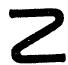
\includegraphics[keepaspectratio]{images/part002_29e6d4b6.jpg}}

注意，R 上的一切有界连续实值函数所成的空间，赋有一致收敛拓扑，不是可数型的（习题 4）。

\subsection{紧开拓扑}

定理 2. 设 X 是拓扑空间，Y 是一致空间。对 X 的每个紧子集 K 及 Y 的每个开子集 U，用 \(\mathbf{T}(\mathbf{K},\mathbf{U})\) 表示一切连续映射 \(u:X\to Y\) （满足 \(u(\mathbf{K})\subset U\) ）所成之集。则诸集 \(\mathbf{T}(\mathbf{K},\mathbf{U})\) 生成 \(\mathcal{C}(\mathbf{X};\mathbf{Y})\) 上的紧收敛拓扑。

设 \(Y'\) 是与 \(Y\) 相伴的豪斯多夫一致空间（第 II 章，§ 3，第 8 号），并设 \(i: Y \to Y'\) 是 \(Y\) 到 \(Y'\) 上的典范映射。紧收敛拓扑是使映射 \(u \to (i \circ u)|K\) （由 \(\mathcal{C}(X; Y)\) 到 \(\mathcal{C}_u(K; Y')\) 中）连续的最粗拓扑，其中 \(K\) 取遍 \(X\) 的一切紧子集所成之集（第 1 节，第 4 号，命题 4）。因此，对 \(\mathcal{C}_c(X; Y)\) 的拓扑，取 \(\mathcal{C}_c(K; Y')\) 的拓扑的一个子基（对每个紧子集 \(K\) ，在 \(X\) 中），再取这些子基的逆像之并{[}在 \(\mathfrak{P}(\mathcal{C}(X; Y))\) 中{]}，逆像取在 \(\mathcal{C}(X, Y)\) 中，便得到它的一个子基。另一方面，\(Y\) 的每个开子集形如 \(\overline{i}^1(U')\) ，其中 \(U'\) 在 \(Y'\) 中开（第 II 章，§ 3，第 7 号，命题 12）；因此，对每个紧子集 \(K' \supset K\) ，\(T(K, \overline{i}^1(U'))\) 是 \(T(K, U')\) 在映射

\[
\mathcal {C} (\mathbf {X}; \mathbf {Y}) \rightarrow \mathcal {C} _ {u} (\mathbf {K} ^ {\prime}; \mathbf {Y} ^ {\prime}).
\]

于是只剩下来证明定理在 X 紧且 Y 豪斯多夫的情形；以下我们就作这些假设。

首先证明 \(T(\mathbf{K}, \mathbf{U})\) 在 \(\mathcal{C}_c(\mathbf{X}; \mathbf{Y})\) 中是开的。设 \(u_0\) 是这个集的一个点；由于 \(u_0(\mathbf{K})\) 紧（第 I 章，§ 9，第 4 号，定理 2 的推论 1）且含于开集 \(\mathbf{U}\) ，存在对称围域 \(\mathbf{V}\) （\(\mathbf{Y}\) 的围域）使 \(\mathbf{V}(u_0(\mathbf{K})) \subset \mathbf{U}\) （第 II 章，§ 4，第 3 号，命题 4 的推论）。设 \(\mathbf{W}\) 是 \(u_0\) 在 \(\mathcal{C}_c(\mathbf{X}; \mathbf{Y})\) 中的由一切连续映射 \(u: \mathbf{X} \to \mathbf{Y}\) （满足 \((u(x), u_0(x)) \in \mathbf{V}\) 对一切 \(x \in \mathbf{K}\) ）组成的邻域。对这些映射我们显然有 \(u(\mathbf{K}) \subset \mathbf{V}(u_0(\mathbf{K})) \subset \mathbf{U}\) ；因此 \(u \in T(\mathbf{K}, \mathbf{U})\) ，从而 \(W \subset T(\mathbf{K}, \mathbf{U})\) ，这就证明了我们的断言。

反之，若 W 是一点 \(u_{0} \in \mathcal{C}_{c}(\mathbf{X}; \mathbf{Y})\) 的邻域，我们要证明 W 含有有限个形如 \(T(\mathbf{K}, \mathbf{U})\) 的邻域的交。可以设 W 是一切 \(u \in \mathcal{C}(\mathbf{X}; \mathbf{Y})\) （满足 \((u(x), u_{0}(x)) \in \mathbf{V}\) 对一切 \(x \in X\) ）所成之集，其中 V 是 Y 的一个给定围域。由于 \(u_{0}\) 在 X 上连续，它一致连续（第 II 章，§ 4，第 1 号，定理 2）。设 \(V_{1}\) 是 Y 的一个对称围域，在 \(Y \times Y\) 中开，且 \(V_{1}^{2} \subset V\) 。X 可被有限个紧集 \(K_{i}\) （ \(1 \leqslant i \leqslant n\) ）覆盖，使得每个 \(u_{0}(\mathbf{K}_{i})\) 是 \(V_{1}\) -小的（ \(1 \leqslant i \leqslant n\) ）。设 \(U_{i}\) 是开集 \(V_{1}(u_{0}(\mathbf{K}_{i}))\) ，并设 \(u: X \to Y\) 是含于 n 个集 \(T(\mathbf{K}_{i}, \mathbf{U}_{i})\) （它们是 \(u_{0}\) 的邻域）之交的一个连续映射。那么，对每个 \(x \in K_{i}\) ，\(u(x)\) 属于 \(U_{i}\) ，因此 \(u_{0}(x)\) 与 \(u(x)\) 是 \(V_{1}^{2}\) -接近的，从而是 V-接近的。由于每个 \(x \in X\) 属于某个 \(K_{i}\) ，我们有 \(u \in W\) ，证明完成。

这个结果引导我们作出如下的定义：

定义 1. 设 X、Y 是两个拓扑空间，不必可一致化。对 X 的每个紧子集 K 及 Y 的每个开子集 U，设 T(K, U) 是一切 \(u \in \mathcal{C}(X; Y)\) （满足 \(u(K) \subset U\) ）所成之集。C(X; Y) 上由诸集 T(K, U) 生成的拓扑称为紧收敛拓扑或紧开拓扑；我们把赋有这个拓扑的 C(X; Y) 所得到的拓扑空间记作 \(\mathcal{C}_{c}(X; Y)\) 。

若 Y 是一致空间，则由定理 2，这个定义与第 1 节第 3 号中给出的定义一致。

若 H 是 \(\mathcal{C}(\mathbf{X};\mathbf{Y})\) 的一个子集，我们把由 \(\mathcal{C}_{c}(\mathbf{X};\mathbf{Y})\) 的拓扑在 H 上诱导的拓扑称为 H 上的紧开拓扑。

例。设 I 是 R 中的区间 \([0, 1]\) 。若 Y 是任一拓扑空间，空间 \(\mathcal{C}_{c}(I; Y)\) 称为 Y 中的道路空间。对每个 \(y \in Y\) ，子空间 \(\Omega_{y}(Y)\) ——\(\mathcal{C}_{c}(I; Y)\) 中由满足 \(u(0) = u(1) = y\) 的道路 u 组成的子空间——称为（Y 中）点 y 处的闭路空间。

注。1) 同样，\(\mathcal{C}(\mathbf{X};\mathbf{Y})\) 上由 \(\mathbf{Y}^{\mathbf{X}} = \mathcal{F}(\mathbf{X};\mathbf{Y})\) 上的乘积拓扑诱导的拓扑称为逐点收敛拓扑（Y 不必可一致化）；它由形如 \(T(\{x\}, \mathbf{U})\) 的集生成，其中 \(x\) 取遍 \(\mathbf{X}\) ，\(\mathbf{U}\) 取遍 \(\mathbf{Y}\) 的一切开子集所成之集，因此它比紧开拓扑粗。由此推出，若 \(\mathbf{Y}\) 豪斯多夫，则空间 \(\mathcal{C}_s(\mathbf{X}; \mathbf{Y})\) 豪斯多夫（第 I 章，§ 8，第 1 号，命题 5 的推论）。

\begin{enumerate}
\def\labelenumi{\arabic{enumi})}
\setcounter{enumi}{1}
\tightlist
\item
  设 \(\mathfrak{S}\) 是 Y 的拓扑的一个子基，并设 \(\mathfrak{R}\) 是 X 的一些紧子集所成之集，具有下列性质：
\end{enumerate}

\begin{enumerate}
\def\labelenumi{(\Alph{enumi})}
\setcounter{enumi}{17}
\tightlist
\item
  若 \(\mathbf{L}\) 是 \(\mathbf{X}\) 的任一紧子集且 \(\mathbf{V}\) 是 \(\mathbf{L}\) 的任一邻域，则存在有限个集 \(\mathbf{K}_i \in \mathfrak{R}\) 使 \(\mathbf{L} \subset \bigcup_{i} \mathbf{K}_i \subset \mathbf{V}\) 。
\end{enumerate}

那么诸集 \(T(\mathbf{K}, \mathbf{U})\) （其中 \(\mathbf{K} \in \mathfrak{R}\) 且 \(\mathbf{U} \in \mathfrak{S}\) ）构成 \(\mathcal{C}(\mathbf{X}; \mathbf{Y})\) 上紧开拓扑的一个子基。为证明这一点，我们必须证明：若 \(\mathbf{L}\) 是 \(\mathbf{X}\) 的任一紧子集且 \(\mathbf{V}\) 是 \(\mathbf{Y}\) 的任一开子集，且 \(u \in T(\mathbf{L}, \mathbf{V})\) ，则存在有限对 \((\mathbf{K}_i, \mathbf{U}_i)\) 使 \(\mathbf{K}_i \in \mathfrak{R}\) 、\(\mathbf{U}_i \in \mathfrak{S}\) 且 \(u \in \bigcap_{i} T(\mathbf{K}_i, \mathbf{U}_i) \subset T(\mathbf{L}, \mathbf{V})\) 。首先注意，对每个有限序列 \((s_k)\) （由 \(\mathfrak{S}\) 中的集合组成）及每个紧子集 \(\mathbf{M}\) （\(\mathbf{X}\) 的子集），由定义我们有 \(T\left(\mathbf{M}, \bigcap_k \mathbf{S}_k\right) = \bigcap_k T(\mathbf{M}, \mathbf{S}_k)\) 。因此我们首先可把 \(\mathfrak{S}\) 换成 \(\mathfrak{S}\) 中集合的有限交所成之集，即我们可设 \(\mathfrak{S}\) 是 \(\mathbf{Y}\) 的拓扑的一个基。由假设，\(u(\mathbf{L})\) 拟紧且含于 \(\mathbf{V}\) ，故存在有限个集 \(\mathbf{U}_i \in \mathfrak{S}\) （含于 \(\mathbf{V}\) ）覆盖 \(u(\mathbf{L})\) 。诸集 \(\overline{u}^1(\mathbf{U}_i)\) 在 \(\mathbf{X}\) 中开且覆盖 \(\mathbf{L}\) 。因此对每个 \(x \in \mathbf{L}\) ，存在紧邻域 \(N_x\) （\(x\) 在 \(\mathbf{L}\) 中的邻域），含于某个 \(\overline{u}^1(\mathbf{U}_i)\) 。\(\mathbf{L}\) 可被有限个这样的集 \(N_{x_j} = L_j\) 覆盖；对每个 \(j\) ，用 \(i(j)\) 表示指标 \(i\) （满足 \(L_j \subset \overline{u}^1(\mathbf{U}_i)\) ）之一。这样，对每个指标 \(j\) 存在{[}由 (R){]}有限个集 \(K_{jk} \subset \overline{u}^1(\mathbf{U}_{i(j)})\) （属于 \(\mathfrak{R}\) ）覆盖 \(L_j\) 。对每个 \(v \in \bigcap_{j,k} T(\mathrm{K}_{jk}, \mathrm{U}_{i(j)})\) 我们有 \(\bigcup_{k} v(\mathrm{K}_{jk}) \subset U_{i(j)}\) ，因此 \(v(\mathrm{L}_j) \subset U_{i(j)}\) ，且 \(v(\mathrm{L}) = \bigcup_{j} v(\mathrm{L}_j) \subset \bigcup_{j} U_{i(j)} \subset V\) ；于是我们的断言得证。

定理 3. 设 X、Y、Z 是三个拓扑空间，并设 f 是 X × Y 到 Z 中的一个映射。若 f 连续，则 \(f: x \to f(x, .)\) 是 X 到 \(\mathcal{C}_{c}(Y; Z)\) 中的一个连续映射。若 Y 局部紧，则逆命题成立。

设 \(f\) 连续。为证明 \(\tilde{f}\) 连续，我们必须证明：对每个紧子集 \(K\) （在 \(Y\) 中）及每个开子集 \(U\) （在 \(Z\) 中），\(V\) （\(T(K, U)\) 在 \(\tilde{f}\) 下的逆像）在 \(X\) 中是开的。设 \(x_0 \in V\) ；对每个 \(y \in K\) ，我们有 \(f(x_0, y) \in U\) ，且由于 \(f\) 连续，存在邻域 \(V_y\) （\(x_0\) 在 \(X\) 中的邻域）及邻域 \(W_y\) （\(y\) 在 \(Y\) 中的邻域）使 \(f(V_y \times W_y) \subset U\) 。由于 \(K\) 紧，存在有限个点 \(y_{i} \in K\) 使诸集 \(W_{y_{i}}(1 \leqslant i \leqslant n)\) 覆盖 K。设 \(V'\) 是诸邻域 \(V_{y_{i}}\) （\(x_{0}\) 的邻域）的交，它是 \(x_{0}\) 的一个邻域；若 \(x \in V'\) 且 \(y \in K\) ，我们有 \(f(x, y) \in U\) ，因为 y 含于某个 \(W_{y_{i}}\) 且 x 含于每个 \(V_{y_{i}}\) ；因此 \(V' \subset V\) ，从而 V 是它的每一点的邻域，于是在 X 中开。

反之，设 \(\tilde{f}\) 连续且 Y 局部紧，我们来证明 \(f\) 连续。设 \(x_0 \in \mathbf{X}\) ，设 \(y_0 \in \mathbf{Y}\) ，并设 U 是 \(f(x_0, y_0)\) 在 Z 中的一个开邻域；我们将证明存在邻域 V （\(x_0\) 在 X 中的邻域）及邻域 W （\(y_0\) 在 Y 中的邻域）使 \(f(\mathbf{V} \times \mathbf{W}) \subset \mathbf{U}\) 。由于 \(y \to f(x_0, y)\) 连续，存在紧邻域 W （\(y_0\) 的邻域）使 \(f(\{x_0\} \times \mathbf{W}) \subset \mathbf{U}\) 。另一方面，由于 \(\tilde{f}\) 连续，集 V （由 \(x \in \mathbf{X}\) 组成，满足 \(f(x, .) \in T(\mathbf{W}, \mathbf{U})\) ）{[}即使 \(f(x, y) \in \mathbf{U}\) 对一切 \(y \in \mathbf{W}]\)是 X 的一个开子集，因而是 \(x_0\) 的一个邻域；且我们有 \(f(\mathbf{V} \times \mathbf{W}) \subset \mathbf{U}\) 。

证毕。

推论 1. 设 X 是局部紧空间，Y 是拓扑空间，H 是 C (X; Y) 的一个子集。则 H 上的紧开拓扑是使映射 \((u, x) \to u(x)\) （由 \(H \times X\) 到 Y 中）连续的最粗拓扑。

因为由定理 3，这个映射连续当且仅当典范单射 \(\mathbf{H} \to \mathcal{C}_c(\mathbf{X}; \mathbf{Y})\) 连续。

注。3) 设 X 是局部紧空间，Y 是豪斯多夫拓扑空间。若 \(\mathcal{G}\) 是 \(\mathcal{C}(\mathbf{X};\mathbf{Y})\) 的一个子集 H 上的一个拓扑，使得映射 \((u,x)\to u(x)\) 在 \(\mathrm{H}\times \mathrm{X}\) 上连续，且 H 关于 \(\mathcal{G}\) 紧，则 \(\mathcal{G}\) 是紧开拓扑。因为由推论 1 它比后者细，且由于紧开拓扑是豪斯多夫的，这两个拓扑相同。注意，若此外 Y 完全正则，则 H 关于与 Y 的拓扑相容的每个一致结构都等度连续（第 2 节，第 5 号，定理 2 的推论 3），且对 X 的每个紧子集 K，集

\[
\mathrm{H} (\mathrm{K}) = \bigcup_ {x \in \mathrm{K}} \mathrm{H} (x)
\]

是紧的，因为它是 \(\mathbf{H} \times \mathbf{K}\) 在连续映射 \((u, x) \to u(x)\) 下的像。

推论 2. 设 X、Y、Z 是三个拓扑空间，使得 X 豪斯多夫且 Y 局部紧。则限制到 \(\mathcal{C}(\mathbf{X} \times \mathbf{Y}; \mathbf{Z})\) 上的典范双射 \(\mathcal{F}(\mathbf{X} \times \mathbf{Y}; \mathbf{Z}) \to \mathcal{F}(\mathbf{X}; \mathcal{F}(\mathbf{Y}; \mathbf{Z}))\) （集合论，R，§4，第 14 号）是 \(\mathcal{C}_c(\mathbf{X} \times \mathbf{Y}; \mathbf{Z})\) 到 \(\mathcal{C}_c(\mathbf{X}; \mathcal{C}_c(\mathbf{Y}; \mathbf{Z}))\) 上的一个同胚。

这个限制当然是一个双射

\[
\rho : \mathcal {C} (\mathrm{X} \times \mathrm{Y}; \mathrm{Z}) \rightarrow \mathcal {C} (\mathrm{X}; \mathcal {C} _ {c} (\mathrm{Y}; \mathrm{Z}))
\]

由定理 3；因此只剩下证明 \(\mathcal{C}(\mathbf{X}\times\mathbf{Y};\mathbf{Z})\) 上的紧开拓扑是 \(\rho\) 下 \(\mathcal{C}(\mathbf{X};\mathcal{C}_{c}(\mathbf{Y};\mathbf{Z}))\) 上紧开拓扑的逆像。由于诸集 \(T(\mathbf{K},\mathbf{U})\) （其中 \(\mathbf{K}\) 是 \(\mathbf{Y}\) 的紧子集且 \(\mathbf{U}\) 是 \(\mathbf{Z}\) 的开子集）构成 \(\mathcal{C}_{c}(\mathbf{Y};\mathbf{Z})\) 的拓扑的一个子基，由注 2 推出，\(\mathcal{C}_{c}(\mathbf{X};\mathcal{C}_{c}(\mathbf{Y};\mathbf{Z}))\) 的拓扑由形如 \(T(J,T(\mathbf{K},\mathbf{U}))\) 的集生成，其中 \(\mathbf{K}\) 与 \(\mathbf{U}\) 如上且 \(J\) 是 \(\mathbf{X}\) 的紧子集。而 \(T(J,T(\mathbf{K},\mathbf{U}))\) 在 \(\rho\) 下的像正是 \(T(J\times K,\mathbf{U})\) ，因此是一个开集；于是我们证明了 \(\rho\) 连续。为证明 \(\rho\) 是一个同胚，我们首先注意形如 \(J\times K\) 的集（在 \(\mathbf{X}\times\mathbf{Y}\) 中）（其中 \(J\) 是 \(\mathbf{X}\) 的紧子集，\(\mathbf{K}\) 是 \(\mathbf{Y}\) 的紧子集）满足注 2 的条件 (R)：因为若 \(\mathbf{L}\) 是 \(\mathbf{X}\times\mathbf{Y}\) 的紧子集且 \(\mathbf{V}\) 是 \(\mathbf{L}\) 在 \(\mathbf{X}\times\mathbf{Y}\) 中的一个邻域，则投影 \(M=pr_{1}(L)\) 、\(N=pr_{2}(L)\) 紧，因为 \(\mathbf{X}\) 与 \(\mathbf{Y}\) 豪斯多夫，且 \(V\cap(M\times N)\) 是 \(\mathbf{L}\) 在紧空间 \(M\times N\) 中的一个邻域，所以 \(\mathbf{L}\) 的每一点在 \(M\times N\) 中有一个形如 \(J\times K\subset V\) （其中 \(J\subset M\) 且 \(K\subset N\) 紧）的邻域；由于 \(\mathbf{L}\) 可被有限个这样的邻域覆盖，断言得证。因此形如 \(T(J\times K;\mathbf{U})\) 的集（其中 \(J\) 是 \(\mathbf{X},\mathbf{K}\) 的紧子集、\(\mathbf{Y}\) 的紧子集，而 \(\mathbf{U}\) 是 \(\mathbf{Z}\) 的开子集）生成 \(\mathcal{C}_{c}(\mathbf{X}\times\mathbf{Y};\mathbf{Z})\) 的拓扑。但我们已经看到 \(T(J\times K,\mathbf{U})\) 在 \(\rho\) 下的像是开集 \(T(J,T(K,\mathbf{U}))\) （在 \(\mathcal{C}_{c}(\mathbf{X};\mathcal{C}_{c}(\mathbf{Y};\mathbf{Z}))\) 中）；因此 \(\rho\) 是一个同胚。

注意，若此外假定 Z 可一致化，则推论 2 是第 1 节第 4 号命题 2 的平凡推论。

命题 9. 设 X、Y、Z 是三个拓扑空间，其中 Y 局部紧。则映射 \((u, v) \to v \circ u\) （由 \(\mathcal{C}_c(X; Y) \times \mathcal{C}_c(Y; Z)\) 到 \(\mathcal{C}_c(X; Z)\) 中）是连续的。

我们必须证明，对 X 的每个紧子集 K 及 Z 的每个开子集 U，由偶 \((u, v)\) （满足 \(v(u(\mathbf{K})) \subset \mathbf{U}\) ）组成的集 R 在 \(\mathcal{C}_{c}(\mathbf{X}; \mathbf{Y}) \times \mathcal{C}_{c}(\mathbf{Y}; \mathbf{Z})\) 中是开的。设 \((u_{0}, v_{0}) \in R\) ；则 \(u_{0}(\mathbf{K})\) 是局部紧空间 Y 的一个紧子集，含于开集 \(\overline{v}_{0}^{1}(\mathbf{U})\) ，因此存在紧邻域 L （\(u_{0}(\mathbf{K})\) 的邻域）含于 \(\overline{v}_{0}^{1}(\mathbf{U})\) （第 I 章，§ 9，第 7 号，命题 10）。集 V （由一切 \(u \in C_{c}(\mathbf{X}; \mathbf{Y})\) （满足 \(u(\mathbf{K}) \subset \mathring{\mathbf{L}}\) ）组成）是 \(u_{0}\) 的一个邻域，而集 W （由一切 \(v \in C_{c}(\mathbf{Y}; \mathbf{Z})\) （满足 \(v(\mathbf{L}) \subset \mathbf{U}\) ）组成）是 \(v_{0}\) 的一个邻域；此外，关系 \((u, v) \in \mathbf{V} \times \mathbf{W}\) 蕴涵 \(v(u(\mathbf{K})) \subset \mathbf{U}\) 。由此即得结论。

\subsection{同胚群上的拓扑}

命题 10. 设 X 是一致空间，H 是 X 到其自身上的同胚所成的一个等度连续集。若 H 与 \(H^{-1}\) 都赋有 X 中逐点收敛的拓扑，则映射 \(u \rightarrow u^{-1}\) （由 \(H^{-1}\) 到 H 上）是连续的。

只需证明，对每个 \(x_0 \in \mathbf{X}\) ，映射 \(u \to u^{-1}(x_0)\) （由 \(\mathbf{H}^{-1}\) 到 \(\mathbf{X}\) 中）在每一点 \(u_0 \in \mathbf{H}^{-1}\) 处连续。设 \(\mathbf{V}\) 是 \(\mathbf{X}\) 的一个对称围域，并设 \(y_0 = u_0^{-1}(x_0)\) 。由假设，存在对称围域 \(\mathbf{U}\) （\(\mathbf{X}\) 的围域），使得关系 \((x, x_0) \in \mathbf{U}\) 蕴涵 \((u^{-1}(x), u^{-1}(x_0)) \in \mathbf{V}\) 对一切 \(u \in \mathbf{H}^{-1}\) 成立。取一个元素 \(u \in \mathbf{H}^{-1}\) ，它是 \(W(\{y_0\}, \mathbf{U})\) -接近于 \(u_0\) 的；则我们有 \((u(y_0), u_0(y_0)) \in \mathbf{U}\) ，即 \((u(y_0), x_0) \in \mathbf{U}\) 。由此得出 \((y_0, u^{-1}(x_0)) \in \mathbf{V}\) ，即 \((u_0^{-1}(x_0), u^{-1}(x_0)) \in \mathbf{V}\) ；证明完成。

推论. 设 X 是一致空间，H 是 X 到其自身上的同胚所成的一个等度连续群。则 X 中逐点收敛的拓扑与 H 的群结构相容。

这是命题 10 连同第 2 节第 1 号命题 1 的推论 5 的推论。

命题 11. 设 X 是紧空间，\(\Gamma\) 是 X 到其自身上的一切同胚所成的群。则 X 中的一致收敛拓扑与 \(\Gamma\) 的群结构相容。

我们已经知道（第 4 号，命题 9）映射 \((u, v) \to v \circ u\) （由 \(\Gamma \times \Gamma\) 到 \(\Gamma\) 中）关于这个拓扑连续；于是只需证明 \(u \to u^{-1}\) 在每一点 \(u_0\) （\(\Gamma\) 的点）处连续。由于 \(u_0^{-1}\) 在 \(\mathbf{X}\) 上一致连续，对任一对称围域 \(\mathbf{V}\) （\(\mathbf{X}\) 的围域），存在一个围域 \(\mathbf{W}\) （\(\mathbf{X}\) 的围域），使得关系 \((x, x') \in \mathbf{W}\) 蕴涵 \((u_0^{-1}(x), u_0^{-1}(x')) \in \mathbf{V}\) 。因此，若 \(u \in \Gamma\) 使 \((u_0(x), u(x)) \in \mathbf{W}\) 对一切 \(x \in \mathbf{X}\) 成立，则得出 \((x, u_0^{-1}(u(x))) \in \mathbf{V}\) 对一切 \(x \in \mathbf{X}\) 成立，从而（由于 \(u\) 是双射）\((u^{-1}(x), u_0^{-1}(x)) \in \mathbf{V}\) 对一切 \(x \in \mathbf{X}\) 成立。证明完成。

\pandocbounded{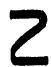
\includegraphics[keepaspectratio]{images/part002_d26bd6ea.jpg}}

现在设 X 是局部紧空间，\(\Gamma\) 是 X 到其自身上的一切同胚所成的群。X 中紧收敛的拓扑不必与 \(\Gamma\) 的群结构相容（习题 17）。用 \(X'\) 表示由 X 添加一个无穷远点 \(\omega\) 所得到的紧空间。X 到其自身上的每个同胚 u 都唯一扩张为一个同胚 \(u'\) （\(X'\) 到其自身上的），使 \(u'(\omega) = \omega\) （第 I 章，§ 10，第 3 号，命题 7 的推论），于是 \(\Gamma\) 可等同于 \(\Gamma'\) （\(X'\) 到其自身上的一切同胚所成的群）中由使 \(\omega\) 不动的一切同胚组成的子群。因此 \(\Gamma\) 上由 \(C_u(X'; X')\) 的拓扑诱导的拓扑与 \(\Gamma\) 的群结构相容（命题 11），且 \(\Gamma\) 在 \(\Gamma'\) 中是闭的{[}关于由 \(\mathcal{C}_u(\mathbf{X}';\mathbf{X}')\) 的拓扑诱导的拓扑{]}，因为它由方程 \(u(\omega)=\omega\) 定义（\(\S\) 1，第 2 号，注 6）。我们用 \(\mathcal{C}_{\beta}\) 表示这样定义在 \(\Gamma\) 上的群拓扑；它比紧收敛的拓扑细，并且也可（借助 \(\S\) 1，第 6 号，命题 6）定义为 \(\mathbf{X}\) 上一致收敛的拓扑，当 \(\mathbf{X}\) 赋有由 \(\mathbf{X}'\) 的唯一一致结构诱导的一致结构时。

拓扑 \(\mathcal{C}_{\beta}\) 可刻画如下：

命题 12. 在群 \(\Gamma\) （局部紧空间 \(\mathbf{X}\) 的一切同胚所成的群）上，拓扑 \(\mathcal{C}_{\beta}\) 是使映射 \(u \to u\) 与 \(u \to u^{-1}\) （由 \(\Gamma\) 到 \(\mathcal{C}_c(\mathbf{X}; \mathbf{X})\) 中）连续的最粗拓扑。

暂把这个拓扑记作 \(\mathcal{C}'\) 。由于 \(u \to u^{-1}\) 关于 \(\mathcal{C}_{\beta}\) 连续，且 \(\mathcal{C}_{\beta}\) 比紧收敛的拓扑细，显然 \(\mathcal{C}_{\beta}\) 比 \(\mathcal{C}'\) 细。为证明其逆，给 \(\mathbf{X}'\) 赋予它的唯一一致结构；设 \(u_0 \in \Gamma\) ，并设 \(\mathbf{V}\) 是 \(\mathbf{X}'\) 的一个围域；于是我们必须证明存在一个紧子集 \(\mathbf{K}\) （\(\mathbf{X}\) 的）与一个对称围域 \(\mathbf{W}\) （\(\mathbf{X}'\) 的），使得关系

\[
u \in \Gamma , (u _ {0} (x), u (x)) \in \mathrm{W} \text {   and   } (u _ {0} ^ {- 1} (x), u ^ {- 1} (x)) \in \mathrm{W} \text {   for   all   } x \in \mathrm{K}
\]

蕴涵

\[
(u _ {0} (x), u (x)) \in \mathbf {V} \text {   for   all   } x \in \mathbf {X}.
\]

设 \(V_1\) 是 \(X'\) 的一个对称开围域，使 \(\dot{V}_1 \subset V\) ；则 \(K_1 = X' - V_1(\omega)\) 是 \(X\) 的一个紧子集。选取一个对称开围域 \(W\) （\(X'\) 的），使 \(W \subset V\) 且 \(W(\omega) \cap W(u_0^{-1}(K_1)) = \emptyset\) ；由第 II 章，§ 4，第 3 号，命题 4，这是可能的。设 \(K_2 = X' - W(\omega)\) ，它是 \(X\) 的一个紧子集。我们将看到 \(W\) 与紧集 \(K = K_1 \cup K_2\) 满足要求。由于 \(W \subset V\) ，只需证明关系

\[
\left(u _ {0} ^ {- 1} (x), u ^ {- 1} (x)\right) \in \mathrm{W} \quad \text { for   all } \quad x \in \mathrm{K} _ {1} \quad (u \in \Gamma)
\]

蕴涵

\[
(u (y), \omega) \in \mathrm{V} _ {1} \quad \text { for   all } \quad y \in \mathrm{W} (\omega);
\]

因为那时我们也将有 \((u_0(y),\omega)\in \mathbf{V}_1\) ，从而

\[
(u _ {0} (y), u (y)) \in \mathring {\mathrm{V}} _ {1} ^ {2} \subset \mathrm{V}
\]

对一切 \(y \in W(\omega) = X' - K_2\) 。现在，若我们有 \(y \in W(\omega)\) 且

\[
u (y) \in \mathrm{X} ^ {\prime} - \mathrm{V} _ {1} (\omega) = \mathrm{K} _ {1},
\]

则将得出 \(y \in u^{-1}(\mathbf{K}_1) \subset W(u_0^{-1}(\mathbf{K}_1))\) ，与 \(W\) 的选取相矛盾；因此证明完成。

一般地，群 \(\Gamma\) （赋有 \(\mathfrak{G}_{\beta}\) ）不是局部紧的；但我们有如下的判别法：

定理 4. 设 G 是局部紧空间 X 的一切同胚所成的群 \(\Gamma\) 的一个子群。假设在空间 \(\mathcal{C}_{\mathfrak{c}}(\mathbf{X};\mathbf{X})\) 中有恒等映射 \(e\) 的一个邻域 V 使 \(\mathbf{V}\cap \mathbf{G} = \mathbf{H}\) 在 G 中对称且在 \(\mathcal{C}_{\mathfrak{c}}(\mathbf{X};\mathbf{X})\) 中相对紧。则闭包 \(\overline{\mathbf{G}}\) （G 在 \(\Gamma\) 中关于拓扑 \(\mathcal{T}_{\beta}\) 的闭包）关于由 \(\mathcal{T}_{\beta}\) 诱导的拓扑是一个局部紧群；在 \(\overline{\mathbf{G}}\) 上诱导的这个拓扑与紧收敛的拓扑相同，且闭包 \(\overline{\mathbf{H}}\) （H 在 \(\mathcal{C}_{\mathfrak{c}}(\mathbf{X};\mathbf{X})\) 中的闭包）是 \(e\) 在 \(\overline{\mathbf{G}}\) 中关于这个拓扑的一个邻域。

首先证明 \(\overline{\mathbf{H}}\) 含于 \(\Gamma\) ，且 \(\overline{\mathbf{H}}\) 上由 \(\mathfrak{C}_{\beta}\) 诱导的拓扑与紧收敛的拓扑相同。设 \(u_0 \in \overline{\mathbf{H}}\) ；于是 \(u_0\) 在 \(\mathcal{C}_c(\mathbf{X}; \mathbf{X})\) 中是超滤子 \(\Phi\) （在 \(\mathbf{H}\) 上）的极限。由于 \(\Phi^{-1}\) （\(\Phi\) 在映射 \(u \to u^{-1}\) 下的像）是 \(\mathbf{H} \subset \overline{\mathbf{H}}\) 上的一个超滤子基，它在紧子空间 \(\overline{\mathbf{H}}\) （\(\mathcal{C}_c(\mathbf{X}; \mathbf{X})\) 的子空间）中收敛于一个元素 \(v_0\) 。映射 \((u, v) \to uv\) 收敛于 \(u_0 v_0\) （关于 \(\Phi \times \Phi^{-1}\) ）（第 4 号，命题 9）；更有甚者，\(u \to uu^{-1} = e\) 收敛于 \(u_0 v_0\) （关于 \(\Phi\) ），故 \(u_0 v_0 = e\) ，因为 \(\mathcal{C}_c(\mathbf{X}; \mathbf{X})\) 豪斯多夫。同样 \(v_0 u_0 = e\) ；于是 \(u_0\) 是 \(\mathbf{X}\) 的一个同胚，即 \(u_0 \in \Gamma\) 。这样 \(\overline{\mathbf{H}}\) 含于 \(\Gamma\) 。此外，这个论证表明 \(\overline{\mathbf{H}}^{-1} = \overline{\mathbf{H}}\) ，且对每个超滤子 \(\Phi\) （在 \(\overline{\mathbf{H}}\) 上，收敛于 \(u_0\) ），\(\Phi^{-1}\) 在 \(\mathcal{C}_c(\mathbf{X}; \mathbf{X})\) 中收敛于 \(u_0^{-1}\) ；因此映射 \(u \to u^{-1}\) （由 \(\overline{\mathbf{H}}\) 到 \(\mathcal{C}_c(\mathbf{X}; \mathbf{X})\) 中）当 \(\overline{\mathbf{H}}\) 带有紧收敛的拓扑时连续（第 I 章，§ 7，第 4 号，命题 9 的推论 1）。于是命题 12 表明，在 \(\overline{\mathbf{H}}\) 上，紧收敛的拓扑与由 \(\mathfrak{C}_{\beta}\) 诱导的拓扑相同。

此外，由于拓扑 \(\mathcal{C}_{\beta}\) （在 \(\Gamma\) 上）比紧收敛的拓扑细，\(\overline{\mathbf{H}}\) 也是 \(\mathbf{H}\) 关于 \(\mathcal{C}_{\beta}\) 的闭包。但 \(\mathbf{H}\) 是 \(e\) 在 \(\mathbf{G}\) 中关于紧收敛的拓扑的一个邻域，从而更是关于由 \(\mathcal{C}_{\beta}\) 诱导的拓扑的邻域；由此（第 I 章，§ 3，第 1 号，命题 2）得出，\(\overline{\mathbf{H}}\) 是 \(e\) 在 \(\overline{\mathbf{G}}\) 中关于由 \(\mathcal{C}_{\beta}\) 诱导的拓扑的一个邻域，因此 \(\overline{\mathbf{G}}\) 关于这个拓扑是局部紧的。若 \(\mathbf{W}\) 是 \(\mathbf{V}\) 关于紧收敛的拓扑的内部，则 \(\mathbf{W} \cap \Gamma\) 在 \(\mathcal{C}_{\beta}\) 中开，因此 \(\mathbf{W} \cap \overline{\mathbf{G}}\) 含于 \(\mathbf{H} = \mathbf{V} \cap \mathbf{G}\) 关于 \(\mathcal{C}_{\beta}\) 的闭包（第 I 章，§ 1，第 6 号，命题 5）；这表明 \(\overline{\mathbf{H}}\) 也是 \(e\) 在 \(\overline{\mathbf{G}}\) 中关于紧收敛的拓扑的一个邻域。最后，对每个 \(u_{0} \in \Gamma\) ，双射 \(v \to u_{0} \circ v\) 与 \(v \to u_{0}^{-1} \circ v\) （由 \(\mathcal{C}_{c}(\mathbf{X}; \mathbf{X})\) 到其自身上）连续（第 4 号，命题 9），因此，若 \(u_{0} \in \overline{G}\) ，则 \(u_{0}\overline{H}\) 是 \(u_{0}\) 在 \(\overline{G}\) 中关于紧收敛的拓扑的一个邻域。证明完成。

推论. 设 G 是局部紧空间 X 的一个同胚群。若闭包 \(\overline{G}\) （G 在 \(\mathcal{C}_{c}(X; X)\) 中的闭包）紧，则 \(\overline{G}\) 是 X 的一个同胚群，且紧收敛的拓扑与 \(\overline{G}\) 的群结构相容，因而它是一个紧拓扑群。

\pandocbounded{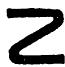
\includegraphics[keepaspectratio]{images/part002_e2b18e11.jpg}}

局部紧空间 X 的一个同胚群，若关于紧收敛的拓扑局部紧但不紧，则由第 I 章，§ 9，第 7 号，命题 12，它在 \(\mathcal{C}_{c}(\mathbf{X};\mathbf{X})\) 中是局部闭的，但不必是闭的。

例如，在环 \(\mathcal{L}(\mathbf{R}^{n})\) （\(\mathbf{R}^{n}\) 的自同态所成的环）中——这个环等同于方阵环 \(\mathbf{M}_{n}(\mathbf{R})\) （\(n \times n\) 方阵，在 \(\mathbf{R}\) 上）且赋有紧收敛的拓扑——，群 \(\mathbf{GL}(n, \mathbf{R})\) （等同于非奇异矩阵所成的群）局部紧但稠密（第 VI 章，§ 1，第 6 号，命题 6）。

\section{连续实值函数的逼近}
